%!TEX root = ../../book_ML.tex

% \chapter{Convex sets và convex functions}
\chapter{Tập lồi và hàm lồi}
\label{cha:convexity}
\index{lồi -- convex}
% \index{convex optimization} 
\section{Giới thiệu}
% Nếu bạn đã đọc các bài trước trong \href{machinelearningcoban.com}{Blog Machine Learning cơ bản}, chúng ta đã làm quen với rất nhiều bài toán tối ưu. Học Machine Learning là phải học Toán Tối Ưu, và để hiểu hơn về Toán Tối Ưu, với tôi cách tốt nhất là tìm hiểu các thuật toán Machine Learning. 
\index{ràng buộc -- constraint}
\index{bài toán tối ưu không ràng buộc -- unconstrained optimization problem}
\subsection{Bài toán tối ưu}
\index{bài toán tối ưu -- convex optimization}
Các bài toán tối ưu đã thảo luận trong cuốn sách này đều là các \textit{bài toán
tối ưu không ràng buộc} ({unconstrained optimization problem}), tức tối
ưu hàm mất mát mà không có \textit{điều kiện ràng buộc} (\textit{constraint})
nào về nghiệm. Tuy nhiên, không chỉ trong machine learning, cài bài 
toán tối ưu trên thực tế thường có rất nhiều ràng buộc khác nhau. 

% Ví dụ

% \begin{itemize}
%     \item Tôi muốn thuê một ngôi nhà cách trung tâm Hà Nội không quá 5km với giá càng thấp càng tốt. Trong bài toán này, giá thuê nhà chính là hàm mất mát (\textit{loss function}, đôi khi người ta cũng dùng \textit{cost function} để chỉ hàm số cần tối ưu), điều kiện khoảng cách không quá 5km chính là ràng buộc (constraint). 
 
%     \item Quay lại \href{http://machinelearningcoban.com/2016/12/28/linearregression/#-gioi-thieu}{bài toán dự đoán giá nhà theo Linear Regression}, giá nhà là một hàm tuyến tính của diện tích, số phòng ngủ và khoảng cách tới trung tâm. Rõ ràng, khi làm bài toán này, ta dự đoán rằng giá nhà tăng theo diện tích và số phòng ngủ, giảm theo khoảng cách. Vậy nên một nghiệm được gọi là \textit{có lý một chút} nếu hệ số tương ứng với diện tích và số phòng ngủ là các số dương, hệ số tương ứng với khoảng cách là một số âm. Để tránh các nghiệm ngoại lai không mong muốn, khi giải bài toán tối ưu, ta nên cho thêm các điều kiện ràng buộc này. 
 
% \end{itemize}

% \newpage
Trong toán tối ưu, một bài toán có ràng buộc thường được viết dưới dạng
\begin{equation}
    \label{eqn:cvxopt_def}
\begin{aligned} 
\mathbf{x}^{*} &=& \arg\min_{\mathbf{x}} f_0(\mathbf{x})\\\ 
\text{thỏa mãn:}~ && f_i(\mathbf{x}) \leq 0, ~~ i = 1, 2, \dots, m \\\ 
&& h_j(\mathbf{x}) = 0, ~~ j = 1, 2, \dots, p 
\end{aligned}
\end{equation} 
 
\index{biến tối ưu -- optimization variable}
\index{tập khả thi -- feasible set}
\index{die@điểm khả thi -- feasible point}
% \index{tập bất khả thi -- infeasible set}
\index{bất phương trình ràng buộc -- inequality constraint}
\index{phương trình ràng buộc -- equality constraint}
\index{hàm bất phương trình ràng buộc -- inequality constraint function}
\index{hàm phương trình ràng buộc -- equality constraint function}
Trong đó, vector $\mathbf{x} = [x_1, x_2, \dots, x_n]^T$ được gọi là
\textit{biến tối ưu} ({optimization variable}). Hàm số $f_0: \mathbb{R}^n
\rightarrow \mathbb{R}$ được gọi là \textit{hàm mục tiêu} (objective function)\footnote{các hàm mục tiêu trong machine learning thường được gọi là
\textit{hàm mất mát}}. 
Các bất phương trình $f_i(\bx) <= 0, i = 1, 2, \dots, m$ được gọi là \textit{bất phương trình ràng buộc} (inequality constraint), và các hàm tương ứng $f_i(\bx), i = 1, 2, \dots, m$ được gọi là \textit{hàm bất phương trình ràng buộc} (inequality constraint function). Các phương trình $h_j(\bx) = 0, j = 1, 2, \dots, p$ được gọi là các \textit{phương trình ràng buộc} (equality constraint), các hàm tương ứng là các \textit{hàm phương trình ràng buộc} (equality constraint function).

\index{tập xác định -- domain}
\def\dom{\boldsymbol{\mathbf{dom}}}
Ký hiệu $\dom f$ là tập các điểm mà trên đó hàm số xác định, hay còn gọi là \textit{tập xác định} (domain). Tập xác định của một bài toán tối ưu là giao của tập xác định tất cả các hàm liên quan:
\begin{equation}
    \mathcal{D} = \bigcap_{i = 0 }^m \dom f_i \cap \bigcap_{j = 0}^p \dom h_j
\end{equation}
Một điểm $\bx \in \mathcal{D}$ được gọi là \textit{điểm khả thi} (feasible point) nếu nó thỏa mãn tất cả ràng buộc: $f_i(\bx) \leq 0, i = 1, 2,\dots, m; h_j(\bx) = 0, j = 1, 2, \dots, p$. Tập hợp các điểm khả thi được gọi là \textit{tập khả thi} (feasible set) hoặc \textit{tập ràng buộc} (constraint set). Như vậy, tập khả thi là một tập con của tập xác định. 
Mỗi điểm trong tập khả thi được gọi là một \textit{điểm khả thi} (feasible point),

Bài toán~\eqref{eqn:cvxopt_def} được gọi là \textit{khả thi} (tương ứng \textit{bất khả thi}) nếu tập khả thi của nó khác (tương ứng bằng) rỗng. 

% các điểm không trong \textit{feasible set} được gọi là các \textit{infeasible
% point}. 

\index{tập khả thi -- feasible set}
\index{die@điểm khả thi -- feasible point}
% \index{tập bất khả thi -- infeasible set}
% \begin{mynote}
\textbf{Chú ý:} 
 \begin{itemize}
    \item Nếu bài toán yêu cầu tìm giá trị lớn nhất thay vì nhỏ nhất của hàm mục
    tiêu, ta chỉ cần đổi dấu của $f_0(\mathbf{x})$.
 
    \item Nếu ràng buộc là {lớn hơn hoặc bằng} ($\geq$), tức $f_i(\mathbf{x}) \geq b_i$, ta chỉ cần đổi dấu của ràng buộc là sẽ có điều kiện \textit{nhỏ hơn hoặc bằng} $-f_i(\mathbf{x}) \leq -b_i$. 
 
    \item Các ràng buộc cũng có thể là {lớn hơn} ($>$) hoặc {nhỏ hơn} ($<$). 
     
    \item Nếu ràng buộc là {bằng nhau}, tức $h_j(\mathbf{x}) = 0$, ta có thể viết nó dưới dạng hai bất phương trình $h_j(\mathbf{x}) \leq 0$ và $-h_j(\mathbf{x}) \leq 0$. 
     
    \item Trong chương này, $\mathbf{x}, \mathbf{y}$ được dùng chủ yếu để ký
    hiệu các biến số, không phải là dữ liệu như trong các chương trước. Các biến cần
    tối được ghi dưới dấu $\arg \min$. Khi viết một bài toán
    tối ưu, ta cần chỉ rõ biến nào cần được tối ưu, biến nào là cố định.
 
\end{itemize}
% \end{mynote}
Nhìn chung, không có cách giải quyết tổng quát cho các bài toán tối ưu, thậm chí
nhiều bài toán tối ưu chưa có lời giải hiểu quả. Hầu hết các phương pháp không
chứng minh được nghiệm tìm được có phải là điểm tối ưu toàn cục hay không. Thay vào đó,
nghiệm thường là các điểm cực trị địa phương. Trong nhiều
trường hợp, các cực trị địa phương cũng mang lại những kết quả tốt.
 
Để bắt đầu nghiên cứu về tối ưu, chúng ta cần biết tới một mảng rất quan trọng có tên là \textit{tối ưu lồi} ({convex optimization}), trong đó
{hàm mục tiêu} là một \textit{hàm lồi} ({convex function}), tập khả thi là một \textit{tập lồi} (convex set). Những tính chất đặc
biệt về cực trị địa phương và toàn cục của một {hàm
lồi} khiến tối ưu lồi trở nên cực kỳ quan trọng. Trong chương này, chúng ta sẽ
thảo luận định nghĩa và các tính chất cơ bản của {tập lồi} và {hàm
lồi}. \textit{Bài toán tối ưu lồi} ({convex optimization problem}) sẽ
được đề cập trong chương tiếp theo.

Trước khi đi sâu vào tập lồi và hàm lồi, xin nhắc lại các hàm liên quan: supremum và infimum. 

\subsection{Các hàm supremum và infimum}

% \index{infimum}
% \index{supremum}
% Xét một hàm số $f: \R^n \rightarrow \R$ với tập xác định $\mathcal{D} \subset \R^n$. Nhắc lại các ký hiệu: 
% \begin{itemize}
%     \item Hàm min: $\displaystyle m = \min_{\bx}f$ nếu $f(\bx) \geq m ~ \forall \bx \in \mathcal{D}$ và $\exists \bx^*\in \mathcal{D}: f(\bx^*) = m$.
%     \item Hàm max: $\displaystyle M = \max_{\bx}f$ nếu $f(\bx) \leq m ~ \forall \bx \in \mathcal{D}$ và $\exists \bx^*\in \mathcal{D}: f(\bx^*) = M$.
%     % \item Hàm inf (infimum) $\displaystyle p = \inf_{\bx}f$ nếu $f(\bx) \geq p ~ \forall \bx \in \mathcal{D}$ và $\forall \varepsilon > 0, \exists \bx_0 \in \mathcal{D}: p \leq f(\bx_0) \leq p + \varepsilon$. Hàm $f(x) = 1/x $ trên tập các số dương có infimum bằng không vì với mọi $\varepsilon > 0, 0 < f(1/varepsilon) = varepsilon$.
% \end{itemize} 
\index{chặn trên -- upper bound}
\index{chặn trên nhỏ nhất -- supremum}.
% \index{không bị chặn trên -- unbounded above}
\index{chặn dưới -- lower bound}
\index{chặn dưới lớn nhất -- infimum}
\def\CC{\mathcal{C}}
Xét một tập $\mathcal{C} \subset \R$. Một số $a$ được gọi là \textit{chặn trên} (upper bound) của $\CC$ nếu   $x \leq a, ~ \forall x \in \CC$. Tập các chặn trên của một tập hợp có thể là tập rỗng, ví dụ $\CC \equiv \R$, toàn bộ $\R$, chỉ khi $\CC = \empty$), hoặc nửa đoạn $[b, +\infty)$. Trong trường hợp cuối, số $b$ được gọi là \textit{chặn trên nhỏ nhất} (supremum) của $\CC$, được ký hiệu là $\sup \CC$. Chúng ta cũng ký hiệu $\sup \empty = -\infty$ và $\sup \CC = +\infty$ nếu $\CC$ \textit{không bị chặn trên} (unbounded above). 

Tương tự, một số $a$ được gọi là \textit{chặn dưới} (lower bound) của $\CC$ nếu $x \geq a, ~\forall x \in \CC$. \textit{Chặn dưới lớn nhất} (infimum) của $\CC$ được ký hiệu là $\inf \CC$. Chúng ta cũng định nghĩa $\inf \empty = +\infty$ và $\inf \CC  = -\infty$ nếu $\CC$ không bị chặn dưới. 

Nếu $\CC$ có hữu hạn số phẩn tử thì $\max \CC = \sup \CC$ và $\min \CC = \inf \CC$.

\index{tập lồi -- convex set}
\section{Tập lồi}
\subsection{Định nghĩa}
Bạn đoc có thể đã biết đến khái niệm \textit{đa giác lồi}. Hiểu một cách đơn giản, \textit{lồi} (convex) là \textit{phình ra ngoài}, hoặc \textit{nhô ra ngoài}. Trong toán học,
{bằng phẳng} cũng được coi là {lồi}.
 
% \myrule 
% \begin{mydef}{Convex sets - Tập hợp lồi (1)}{cvxset}
\textit{\textbf{Định nghĩa không chính thức của tập lồi}}: Một tập hợp được gọi là
\textit{tập lồi} (convex set) nếu mọi điểm trên đoạn thẳng nối hai điểm {bất kỳ} trong
nó đều thuộc tập hợp đó.

% \end{mydef}
% \myrule 

\begin{figure}[t]
\centering
    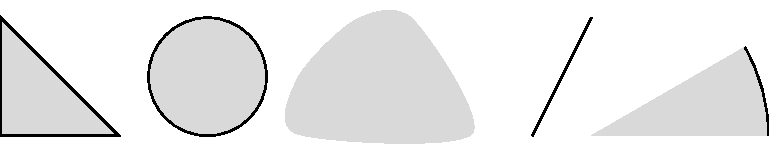
\includegraphics[width = .8\textwidth]{Chapters/08_ConvexOptimization/16_convexity/latex/convexsets.pdf}
    \caption[]{Các ví dụ về tập lồi}
    \label{fig:16_convexsets}
\end{figure}

Một vài ví dụ về tập lồi được cho trong Hình \ref{fig:16_convexsets}. Các hình
với đường biên màu đen thể hiện việc biên cũng thuộc vào hình đó, biên màu trắng
thể hiện việc biên đó không nằm trong hình. Đường thẳng hoặc đoạn
thẳng cũng là một tập lồi theo định nghĩa phía trên.
 
Một vài ví dụ thực tế: 

\begin{itemize}
    \item Giả sử một căn phòng có dạng hình lồi, nếu ta đặt một bóng đèn đủ
    sáng ở bất kỳ vị trí nào trên trần nhà, mọi điểm trong căn phòng đều được
    chiếu sáng.
 
    \item Nếu một đất nước có bản đồ dạng hình lồi thì đoạn thẳng nối hai
    thành phố bất kỳ của đất nước đó nằm trọn vẹn trong lãnh thổ của nó. Một cách lý
    tưởng, mọi đường bay trong đất nước đều được tối ưu vì chi phí bay thẳng ít
    hơn chi phí bay vòng hoặc qua không phận của nước khác. Bản đồ Việt
    Nam không có dạng lồi vì đường thẳng nối sân bay Nội Bài và Tân Sơn Nhất đi
    qua địa phận Campuchia. 

\end{itemize}
 
 
% \myrule  
% <div class="imgcap"> 
%  <img src ="/assets/16_convexity/nonconvexsets.png" align = "center" width = "800"> 
%  <div class = "thecap">Hình 2: Các ví dụ về nonconvex sets.</div> 
% </div> 
% \myrule  

\begin{figure}[t]
\centering
    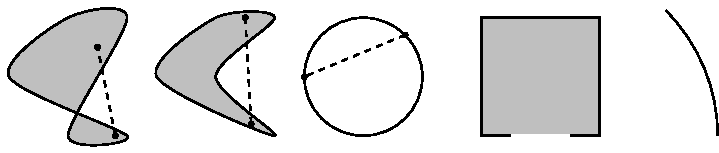
\includegraphics[width = .8\textwidth]{Chapters/08_ConvexOptimization/16_convexity/latex/nonconvexsets.pdf}
    \caption[]{Các ví dụ về tập không lồi.}
    \label{fig:16_nonconvexsets}
\end{figure}

\index{tập không lồi -- nonconvex set}
Hình \ref{fig:16_nonconvexsets} minh hoạ một vài ví dụ về các tập không phải là
tập lồi, nói gọn là \textit{tập không lồi} ({nonconvex set}). Ba hình đầu
tiên không phải lồi vì các đường nét đứt chứa nhiều điểm không nằm bên trong các
tập đó. Hình thứ tư, hình vuông không có biên ở đáy, là tập không lồi vì đoạn thẳng nối hai điểm ở đáy có thể chứa phần ở giữa không
thuộc tập đang xét. Một đường cong
bất kỳ cũng là tập không lồi vì đường thẳng nối hai điểm
bất kỳ không thuộc đường cong đó.
 
Để mô tả một {tập lồi} dưới dạng toán học, ta sử dụng:

\begin{mydef}{Tập hợp lồi}{cvxset2}
Một tập hợp $\mathcal{C}$ được gọi là một {\textit{tập lồi}} (convex set) nếu với hai điểm bất
kỳ $\mathbf{x}_1, \mathbf{x}_2 \in \mathcal{C}$, điểm $ \mathbf{x}_{\theta} =
\theta \mathbf{x}_1 + (1 - \theta) \mathbf{x}_2$ cũng nằm trong $\mathcal{C}$
với $0 \leq \theta \leq 1$.
\end{mydef}

Tập hợp các điểm có dạng $\left(\theta \mathbf{x}_1 + (1 -
\theta) \mathbf{x}_2\right)$ chính là {đoạn thẳng} nối hai điểm
$\mathbf{x}_1$ và $\mathbf{x}_2$.
 
Với định nghĩa này, {toàn bộ không gian} là một {tập lồi}
vì đoạn thằng nào cũng nằm trong không gian đó. Tập rỗng cũng có thể coi là một
trường hợp đặc biệt của {tập lồi}.
 
% Dưới đây là một vài ví dụ hay gặp về \textit{tập lồi}. 
% \newpage  
\subsection{Các ví dụ về tập lồi}

\textit{\textbf{{Siêu mặt phẳng} và {nửa không gian}}}
\index{siêu mặt phẳng -- hyperplane}
\begin{mydef}{Siêu mặt phẳng}{hyperplane}
Một \textit{siêu mặt phẳng}, hay \textit{siêu phẳng} ({hyperplane}) trong
không gian $n$ chiều là tập hợp các điểm thỏa mãn phương trình
\begin{equation} 
a_1 x_1 + a_2 x_2 + \dots + a_n x_n = \mathbf{a}^T\mathbf{x} = b 
\end{equation} 
với $b, a_i, i = 1, 2, \dots, n$ là các số thực. 
\end{mydef}
 
Siêu phẳng là các {tập lồi}. Điều này có thể được suy ra từ Định
nghĩa~\ref{def:cvxset2}. Thật vậy, nếu
\begin{equation*} 
\mathbf{a}^T\mathbf{x}_1 = \mathbf{a}^T\mathbf{x}_2 = b 
\end{equation*} 
thì với $0 \leq \theta \leq 1$ bất kỳ, ta có 
\begin{math} 
\mathbf{a}^T\mathbf{x}_{\theta} = \mathbf{a}^T(\theta \mathbf{x}_1 + (1 - \theta)\mathbf{x}_2) = \theta b + (1 - \theta) b  = b. 
\end{math} 
Tức là $\theta \bx_1 + (1 - \theta)\bx_2$ cũng là một điểm thuộc siêu phẳng đó. 
\index{nửa không gian -- halfspace}
\begin{mydef}{Nửa không gian}{halfspace}
    Một \textit{nửa không gian} ({halfspace}) trong không gian $n$ chiều là
    tập hợp các điểm thỏa mãn bất phương trình
    \begin{equation*} 
    a_1 x_1 + a_2 x_2 + \dots + a_n x_n = \mathbf{a}^T\mathbf{x} \leq b 
    \end{equation*} 
    với $b, a_i, i = 1, 2, \dots, n$ là các số thực. 
\end{mydef}
 
Các nửa không gian cũng là các tập lồi, bạn đọc có thể kiểm tra theo Định
nghĩa~\ref{def:cvxset2} và cách chứng minh tương tự như trên. 
 
\index{cầu chuẩn -- norm ball}
\textit{\textbf{Cầu chuẩn}}
\begin{mydef}{Cầu chuẩn}{euball}
    Cho một tâm $\bx_c$, một bán kính $r$ và khoảng cách giữa các điểm được
    xác định bởi một chuẩn. \textit{Cầu chuẩn} (norm ball) tương ứng là tập hợp các điểm thoả
    mãn 
    \begin{equation*}
    B(\mathbf{x}_c, r) = \left\{\mathbf{x} ~\big|~ \|\mathbf{x} - \mathbf{x}_c\| \leq r \} = \{\mathbf{x}_c + r\mathbf{u} ~\big|~ \|\mathbf{u}\| \leq 1\right\} 
    \end{equation*} 
\end{mydef}
Khi chuẩn là $\ell_2$, cầu chuẩn là một hình tròn trong không gian hai chiều,
hình cầu trong không gian ba chiều, hoặc siêu cầu trong các không gian nhiều
chiều. %Khi dùng chuẩn $\ell_2$, cầu chuẩn được gọi là \textit{Euclidean norm}. 

Cầu chuẩn là tập lồi. Để chứng minh việc này, ta dùng Định nghĩa~\ref{def:cvxset2} và
bất đẳng thức tam giác của chuẩn. Với $\mathbf{x}_1, \mathbf{x}_2$ bất kỳ thuộc
$B(\mathbf{x}_c, r)$ và $0 \leq \theta \leq 1$ bất kỳ, xét $\bx_{\theta} =
\theta \bx_1 + (1 - \theta)\bx_2$, ta có: 
% \begin{equation*} 
\begin{eqnarray*} 
\|\mathbf{x}_{\theta} - \mathbf{x}_c\| &=& \|\theta(\mathbf{x}_1 - \mathbf{x}_c)  + (1 - \theta) (\mathbf{x}_2 - \mathbf{x}_c)\| \\\ 
&\leq& \theta \|\mathbf{x}_1 - \mathbf{x}_c\| + (1 - \theta)\|\mathbf{x}_2 - \mathbf{x}_c\| 
\leq \theta r + ( 1 - \theta) r = r 
\end{eqnarray*} 
% \end{equation*} 
Vậy $\mathbf{x}_{\theta} \in B(\mathbf{x}_c, r)$. 
 
% \textbf{Euclidean ball} sử dụng $\ell_2$ norm làm khoảng cách. Nếu sử dụng norm bất kỳ là khoảng cách, ta vẫn được một \textit{tập lồi}. 
 

% \textbf{Khi sử dụng norm $p$} bất kỳ, ta có  
% \begin{equation*} 
% \|\mathbf{x}\|_p = (\|x_1\|^p + \|x_2\|^p + \dots \|x_n\|^p)^{\frac{1}{p}}
% \end{equation*} 
% với \textbf{p là một số thực bất kỳ không nhỏ hơn 1} ta cũng thu được các \textit{tập lồi}. 
 
\begin{figure}[t]
\centering
    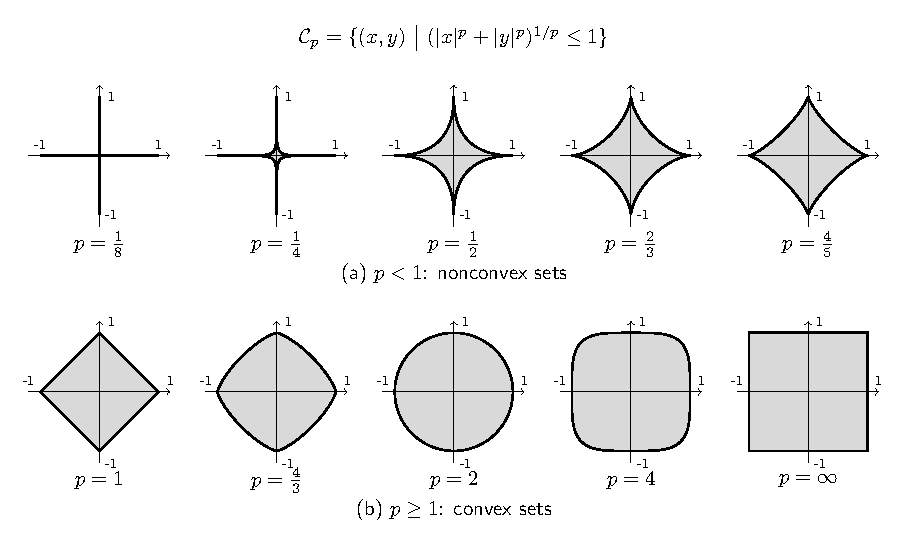
\includegraphics[width = \textwidth]{Chapters/08_ConvexOptimization/16_convexity/latex/normballs.pdf}
    \caption[]{Hình dạng của các tập hợp bị chặn bởi  các (a) giả chuẩn và
    (b) chuẩn.} \label{fig:16_normballs}
\end{figure}

\index{giả chuẩn -- pseudo norm}
Hình \ref{fig:16_normballs} minh họa tập hợp các điểm có tọa độ $(x, y)$ trong không gian hai chiều thỏa mãn: 
\begin{equation} 
\label{eqn:16_normp}
(|x|^p + |y|^p)^{1/p} \leq 1 
\end{equation} 
Hàng trên là các tập tương ứng $0 < p < 1$ là các giả chuẩn; hàng dưới tương
ứng $p \geq 1$ là các chuẩn thực sự. Có thể thấy rằng khi $p$ nhỏ
gần bằng không, tập hợp các điểm thỏa mãn bất đẳng thức \eqref{eqn:16_normp} gần như
nằm trên các trục tọa độ và bị chặn trong đoạn $[0, 1]$. Quan sát này sẽ giúp
ích khi làm việc với giả chuẩn $\ell_0$. Khi $p \rightarrow
\infty$, các tập hợp hội tụ về hình vuông.
Đây cũng là một trong các lý do vì sao cần có điều kiện $p \geq 1$ khi định
nghĩa chuẩn $\ell_p$. 
 
% \textbf{Ellipsoids} 
% \index{ellipsoids} 

% Các ellipsoids (ellipse trong không gian nhiều chiều) cũng là các \textit{tập
% lồi}. Thực chất, ellipsoides có mối quan hệ mật thiết tới
% \href{https://en.wikipedia.org/wiki/Mahalanobis_distance}{Khoảng cách
% Mahalanobis}. Khoảng cách này vốn dĩ là một norm nên ta có thể chứng minh theo
% Định nghĩa 2 được tính chất lồi của các ellipsoids.

% \index{Mahalanobis norm}
% \textbf{Mahalanobis norm} của một vector $\mathbf{x} \in \mathbb{R}^n$ được định nghĩa là: 
% \begin{equation*} 
% \|\mathbf{x}\|_{\mathbf{A}} = \sqrt{\mathbf{x}^T\mathbf{A}^{-1}\mathbf{x}} 
% \end{equation*} 
 
% Với $\mathbf{A}^{-1}$ là một ma trận thỏa mãn: 
% \begin{equation} 
% \label{eqn:16_mahnorm}
% \mathbf{x}^T\mathbf{A}^{-1}\mathbf{x} \geq 0, ~~\forall \mathbf{x} \in \mathbb{R}^n
% \end{equation} 
% Khi một ma trận $\mathbf{A}^{-1}$ thỏa mãn điều kiện \eqref{eqn:16_mahnorm}, ta nói ma trận đó \textit{xác định dương} (\textit{positive definite}). Một ma trận là \textit{xác định dương} nếu các {trị riêng} (eigenvalues) của nó là dương. 
 
% Nhân tiện, một ma trận $\mathbf{B}$ được gọi là \textbf{nửa} \textit{xác định dương} (\textit{positive semidefinite}) nếu các \textit{trị riêng} của nó là không âm. Khi đó $\mathbf{x}^T \mathbf{Bx} \geq 0, \forall \mathbf{x}$. Nếu dấu bằng xảy ra khi và chỉ khi $\mathbf{x} = 0$ thì ta nói ma trận đó \textit{xác định dương}. Trong biểu thức \eqref{eqn:16_mahnorm}, vì ma trận $\mathbf{A}$ có nghịch đảo nên mọi \textit{trị riêng} của nó phải khác không. Vì vậy, $\mathbf{A}$ là một ma trận \textit{xác định dương}. 
 
% Một ma trận $\mathbf{A}$ là \textit{xác định dương} hoặc \textit{nửa xác định dương} sẽ được ký hiệu lần lượt như sau: 
% \begin{equation*} 
% \mathbf{A} \succ 0, ~~~~~ \mathbf{A} \succeq 0. 
% \end{equation*} 
 
% Cũng lại nhân tiện, khoảng cách Mahalanobis có liên quan đến \textit{khoảng cách từ một điểm tới một phân phối xác suất} (from a point to a distribution).  
 
\subsection{Giao của các tập lồi}
Giao của các tập lồi là một tập lồi. Điều này có thể nhận thấy trong Hình
\ref{fig:16_intersection}a. Giao của hai trong ba hoặc cả ba tập lồi đều là các
tập lồi. Điều này có thể được chứng minh theo Định nghĩa~\ref{def:cvxset2}: nếu
$\mathbf{x}_1, \mathbf{x}_2$ thuộc giao của các tập lồi thì $(\theta\mathbf{x}_1 + (1 - \theta) \mathbf{x}_2)$ cũng thuộc giao của chúng.
 
% <hr> 
% <div class="imgcap"> 
%  <img src ="/assets/16_convexity/intersection.png" align = "center" width = "800"> 
%  <div class = "thecap">Hình 4. Trái: Giao của các tập lồi là một tập lồi. Phải: giao của các hyperplanes và halfspace là một tập lồi và được gọi là polyhedron (số nhiều là polyhedra).</div> 
% </div> 
% <hr> 
\begin{figure}[t]
\centering
    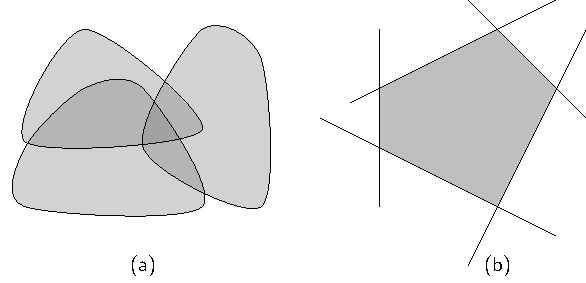
\includegraphics[width = .6\textwidth]{Chapters/08_ConvexOptimization/16_convexity/latex/intersection.pdf}
    \caption[]{(a) Giao của các tập lồi là một tập lồi. (b) Giao của các
    siêu phẳng và nửa không gian là một tập lồi và được gọi là \textit{siêu đa diện} (polyhedra).}
    \label{fig:16_intersection}
\end{figure}

\index{siêu đa diện -- polyhedra}
Từ đó suy ra giao của các nửa không gian và nửa mặt phẳng
là một tập lồi. Chúng là các đa giác lồi trong không gian hai chiều, đa
diện lồi trong không gian ba chiều, và \textit{siêu đa diện} trong không gian nhiều chiều.
Giả sử có $m$ nửa không gian và $p$ siêu phẳng. Mỗi nửa không gian có thể được viết dưới dạng $\mathbf{a}_i^T\mathbf{x} \leq
b_i, ~\forall i = 1, 2, \dots, m$. Một siêu phẳng có thể được viết
dưới dạng $\mathbf{c}_i^T\mathbf{x} = d_i, ~\forall i = 1, 2, \dots, p$.
 
Vậy nếu đặt $\mathbf{A} = [\mathbf{a}_1, \mathbf{a}_2, \dots, \mathbf{a}_m]$,
$\mathbf{b} = [b_1, b_2, \dots, b_m]^T, \mathbf{C} = [\mathbf{c}_1,
\mathbf{c}_2, \dots, \mathbf{c}_p]$ và $\mathbf{d} = [d_1, d_2, \dots, d_p]^T$, ta
có thể viết siêu đa diện dưới dạng tập hợp các điểm $\mathbf{x}$ thỏa mãn
\begin{equation*} 
 \mathbf{A}^T\mathbf{x} \preceq \mathbf{b}, ~~~~  \mathbf{C}^T\mathbf{x} = \mathbf{d} 
\end{equation*} 
trong đó $\preceq$ thể hiện mỗi phần tử trong vế trái nhỏ
hơn hoặc bằng phần tử tương ứng trong vế phải.
 

\index{tổ hợp lồi -- convex combination}
\subsection{Tổ hợp lồi và bao lồi}
\begin{mydef}{Tổ hợp lồi}{}
    Một điểm được gọi là \textit{tổ hợp lồi} ({convex combination}) của các
    điểm $\mathbf{x}_1, \mathbf{x}_2, \dots, \mathbf{x}_k$ nếu nó có thể được viết dưới dạng
    \begin{equation*} 
    \mathbf{x} = \theta_1 \mathbf{x}_1 + \theta_2 \mathbf{x}_2 + \dots  +
    \theta_k \mathbf{x}_k ~~ \text{với} ~~ \theta_1 + \theta_2 + \dots +
    \theta_k = 1 ~\text{và}~ \theta_i \geq 0, \forall i= 1, 2, \dots, k 
    \end{equation*} 
\end{mydef}

\index{bao lồi -- convex hull}
\textit{Bao lồi} ({{convex hull}}) của một {tập bất kỳ} là tập
toàn bộ các tổ hợp lồi của tập hợp đó.
Bao lồi của một tập bất kỳ là một tập lồi.
Bao lồi của một tập lồi là chính nó. Bao lồi của một tập hợp là tập lồi {nhỏ nhất} chứa tập
hợp đó. Khái niệm {\textit{nhỏ nhất}} được hiểu là mọi tập lồi chứa toàn bộ các tổ hợp lồi đều chứa bao lồi của tập hợp đó. 
 
\index{tách biệt tuyến tính -- linearly separable}

Nhắc lại khái niệm \textit{tách biệt tuyến tính} đã sử dụng nhiều trong cuốn
sách. Hai tập hợp được gọi là tách biệt tuyến tính nếu bao lồi của chúng không giao nhau.

\begin{figure}[t]
\centering
    % \rulecaption
    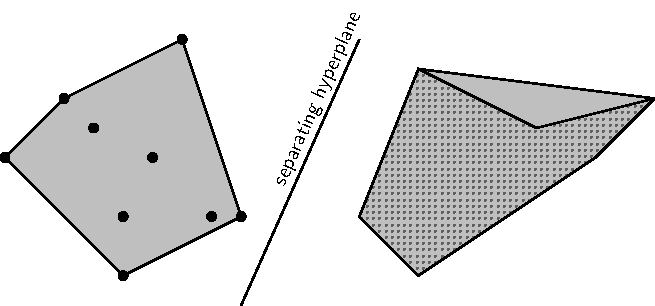
\includegraphics[width = .7\textwidth]{Chapters/08_ConvexOptimization/16_convexity/latex/convex_hull.pdf}
    \caption[]{Trái: Bao lồi của các điểm màu đen là đa giác lồi nhỏ nhất chứa toàn bộ các điểm này. Phải: Bao lồi của đa giác lõm nền chấm là hợp của nó và tam giác màu xám phía trên. Hai bao lồi không giao nhau này có thể được phân tách hoàn toàn bằng một siêu phẳng (trong trường hơp này là một đường thẳng).}
    \label{fig:16_convex_hull}
    \captionsetup[figure]{format=rule, justification=centering}
    % \myrule
\end{figure}


Trong Hình \ref{fig:16_convex_hull}, bao lồi của các điểm màu đen là vùng
màu xám bao bởi các đa giác lồi. Trong Hình \ref{fig:16_convex_hull} bên phải,
bao lồi của đa giác lõm nền chấm là hợp của nó và phần tam giác màu xám. 

\index{din@định lý siêu phẳng phân chia -- separating hyperplane theorem}
\begin{mytheo}{Siêu phẳng phân chia}{sephyper}
Hai {tập lồi không rỗng} $\mathcal{C}, \mathcal{D}$  {không giao
nhau} khi và chỉ khi tồn tại một vector $\mathbf{a}$ và một số $b$ sao cho
\begin{equation*} 
\mathbf{a}^T\mathbf{x} \leq b, \forall \mathbf{x} \in \mathcal{C}, ~~ \text{}~~ \mathbf{a}^T\mathbf{x} \geq b, \forall \mathbf{x} \in \mathcal{D} 
\end{equation*} 

Tập hợp tất cả các điểm $\mathbf{x}$ thỏa mãn $\mathbf{a}^T\mathbf{x} = b$ là một siêu phẳng. Siêu phẳng này được gọi là \textit{siêu phẳng phân chia} ({separating hyperplane}). 
\end{mytheo}

Ngoài ra, còn nhiều tính chất thú vị của các tập lồi và các phép toán bảo toàn
chính chất {lồi} của một tập hợp, bạn đọc có thể đọc thêm
Chương 2 của cuốn \textit{Convex Optimization}~\cite{boyd2004convex}.
 
 
\section{Hàm lồi}
 
% Hẳn các bạn đã nghe tới khái niệm này khi ôn thi đại học môn toán. Khái niệm hàm lồi có quan hệ tới đạo hàm bậc hai và \href{https://vi.wikipedia.org/wiki/Bất_đẳng_thức_Jensen}{Bất đẳng thức Jensen} (\textit{nếu bạn chưa nghe tới phần này, không sao, bây giờ bạn sẽ biết}). 
 
 
\subsection{Định nghĩa}
% \index{convex!function!domain}
\index{hàm lồi -- convex function}
Trước hết ta xem xét các hàm một biến với đồ thị của nó là một đường trong một
mặt phẳng. Một hàm số được gọi là \textit{lồi} (convex) nếu {tập xác định của nó
là một tập lồi} và đoạn thẳng nối hai điểm bất kỳ trên đồ thị hàm số đó nằm về phía trên hoặc nằm trên đồ thị (xem
Hình~\ref{fig:16_convexf_def}). 
\begin{mydef}{Hàm lồi}{cvxfun}
    Một hàm số $f: \mathbb{R}^n \rightarrow \mathbb{R} $ được gọi là một \textit{hàm lồi} (convex function) nếu $\textbf{dom} f$ là một {tập lồi}, và: 
\begin{equation*} 
f(\theta\mathbf{x} + (1 - \theta) \mathbf{y}) \leq \theta f(\mathbf{x}) + (1 - \theta)f(\mathbf{y}) 
\end{equation*} 
với mọi $\mathbf{x, y} \in \textbf{dom}f, 0 \leq \theta \leq 1$. 
\end{mydef}


Điều kiện $\textbf{dom} f$ là một {tập lồi} rất quan trọng. Nếu không
có điều kiện này, tồn tại những $\theta$ mà $\theta \bx_1 + (1-\theta)\bx_2$
không thuộc $\dom f$ và $f(\theta\mathbf{x} + (1 -
\theta)
\mathbf{y}) $ không xác định.
 
% <hr> 
% <div class="imgcap"> 
%  <img src ="/assets/16_convexity/convexf_def.png" align = "center" width = "500"> 
%  <div class = "thecap">Hình 5. Convex function.</div> 
% </div> 
% <hr> 
% \begin{figure}[t]
% \centering
%     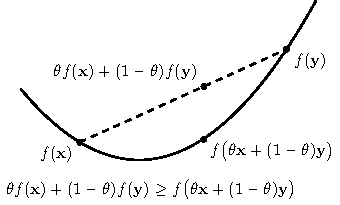
\includegraphics[width = .5\textwidth]{Chapters/08_ConvexOptimization/16_convexity/latex/convexf_def.pdf}
%     \caption[]{Định nghĩa hàm lồi. Diễn đạt bằng lời, một hàm số là lồi nếu đoạn thẳng nối 2 điểm bất kỳ trên đồ thị của nó \textit{không nằm dưới} đồ thị đó. }
%     \label{fig:16_convexf_def}
% \end{figure}

\begin{figure}[t]
    % caption on side     
    \floatbox[{\capbeside\thisfloatsetup{capbesideposition={right,top},capbesidewidth=6cm}}]{figure}[\FBwidth]
    {\caption{Định nghĩa hàm lồi. Diễn đạt bằng lời, một hàm số là lồi nếu đoạn thẳng nối hai điểm bất kỳ trên đồ thị của nó {không nằm phía dưới} đồ thị đó. }
    \label{fig:16_convexf_def}}
    {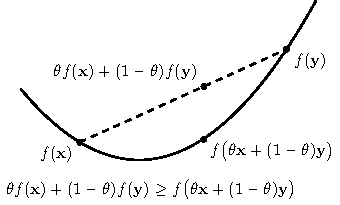
\includegraphics[width=8cm]{Chapters/08_ConvexOptimization/16_convexity/latex/convexf_def.pdf}}
    % \myrule
\end{figure}


% \begin{SCfigure}
%     \caption{Định nghĩa hàm lồi. Diễn đạt bằng lời, một hàm số là lồi nếu đoạn thẳng nối 2 điểm bất kỳ trên đồ thị của nó \textit{không nằm dưới} đồ thị đó.}
%     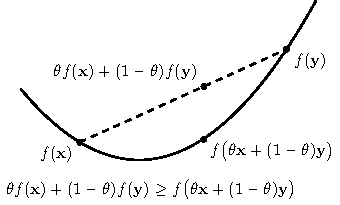
\includegraphics[width=7cm]{Chapters/08_ConvexOptimization/16_convexity/latex/convexf_def.pdf}

% \end{SCfigure}
\index{hàm lõm -- concave function}
Một hàm số $f$ được gọi là \textit{hàm lõm} (concave fucntion) nếu $-f$
là một hàm lồi. Một
hàm số có thể không thuộc hai loại trên. Các hàm tuyến tính vừa lồi vừa lõm.
% \index{convex!strictly convex functions}
\index{hàm lồi chặt -- stricly convex function}
\begin{mydef}{Hàm lồi chặt}{strictlycvx}
 Một hàm số $f: \mathbb{R}^n \rightarrow \mathbb{R} $ được gọi là
 \textit{hàm lồi chặt} ({strictly convex function}) nếu $\dom f$ là một
 {tập lồi}, và
\begin{equation*} 
f(\theta\mathbf{x} + (1 - \theta) \mathbf{y}) < \theta f(\mathbf{x}) + (1 - \theta)f(\mathbf{y}) 
\end{equation*} 
 $\forall~\mathbf{x, y} \in \text{dom}f, \mathbf{x} \neq \mathbf{y},  0 < \theta
< 1$ (chỉ khác hàm lồi ở dấu nhỏ hơn).

\end{mydef}

\index{hàm lõm chặt -- stricly concave function}
Tương tự với định nghĩa \textit{hàm lõm chặt} (stricly concave function). 
 
\textit{Nếu một hàm số là \textit{lồi chặt} và có điểm cực trị, thì điểm cực trị đó là duy nhất và cũng là cực trị toàn cục}. 
 
 
\subsection{Các tính chất cơ bản}
\label{ssub:16_properties}
\begin{itemize}
    \item Nếu $f(\mathbf{x})$ là một hàm lồi thì $af(\mathbf{x})$ cũng lồi khi $a > 0$ và lõm khi $a < 0$. Điều này có
    thể suy ra trực tiếp từ định nghĩa.
     
    \item Tổng của hai {hàm lồi} là một {hàm lồi}, với tập xác
    định là giao của hai tập xác định của hai hàm đã cho (nhắc lại rằng giao của
    hai tập lồi là một tập lồi).
    \index{supremum}
    \item {Hàm max và sup tại từng điểm}: Nếu các hàm số $f_1, f_2,
    \dots, f_m$ lồi thì
    \begin{equation*} 
    f(\mathbf{x}) = \max\{f_1(\mathbf{x}), f_2(\mathbf{x}), \dots, f_m(\mathbf{x})\} 
    \end{equation*} 
    cũng là lồi trên $\displaystyle \dom f = \bigcap_{i=1}^m \dom f_i$. Hàm $\max$ cũng có thể thay thế bằng hàm
    {sup}. Tính chất này có thể được chứng minh theo
    Định nghĩa~\ref{def:cvxfun}. Hình~\ref{fig:16_max_point} minh hoạ tính chất
    này. Các hàm $f_1(\bx), f_2(\bx)$ là các hàm lồi. Đường nét đậm chính là đồ
    thị của hàm số $f(\bx) = \max(f_1(\bx), f_2(\bx))$. Mọi đoạn thẳng nối hai
    điểm bất kì trên đường này đều {không nằm phía dưới} nó.
 
\end{itemize}

\begin{figure}[t]
    % caption by side
    \floatbox[{\capbeside\thisfloatsetup{capbesideposition={right,top},capbesidewidth=7cm}}]{figure}[\FBwidth]
    {\caption{Ví dụ về Pointwise maximum. Maximum của các hàm lồi là một hàm lồi.}
    \label{fig:16_max_point}}
    {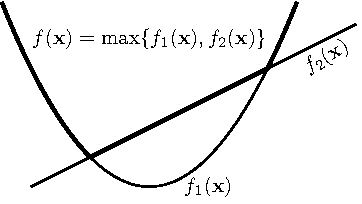
\includegraphics[width=7cm]{Chapters/08_ConvexOptimization/16_convexity/latex/max_point.pdf}}
\end{figure}


\subsection{Ví dụ}
 
\subsubsection{Các hàm một biến}
% \textbf{Ví dụ về các \textit{convex functions} một biến:} 
Ví dụ về hàm lồi:
\begin{itemize}
    \item Hàm $ y = ax + b$ là một {hàm lồi} vì đoạn thẳng nối hai điểm
    bất kỳ trên đường thẳng đó đều {không nằm phía dưới} đường thẳng đó. 
     
    \item Hàm $y = e^{ax}$ với $a \in \mathbb{R}$ bất kỳ. 
     
    \item Hàm $y = x^a$ trên tập các số thực dương và $a \geq 1$ hoặc $a \leq 0$. 
     
    \item Hàm \textit{entropy âm} (negative entropy) $y = x \log x$ trên tập các số thực dương. 

\end{itemize}
 
Hình \ref{fig:16_convexfunctions} minh hoạ đồ thị của một số hàm lồi thường
gặp với biến một chiều.
% <hr> 
% <div class="imgcap"> 
%  <img src ="/assets/16_convexity/convexfunctions.png" align = "center" width = "800"> 
%  <div class = "thecap">Hình 7. Ví dụ về các convex functions một biến.</div> 
% </div> 
% <hr> 

\begin{figure}[t]
\myrule
\vspace{3mm}
\centering
    % \rulecaption
    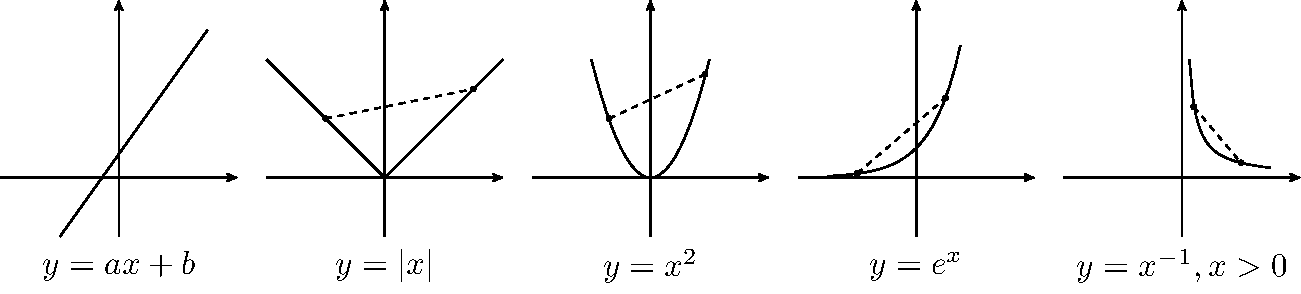
\includegraphics[width = \textwidth]{Chapters/08_ConvexOptimization/16_convexity/latex/convexfunctions.pdf}
    \caption[]{Ví dụ về các hàm lồi một biến.}
    \label{fig:16_convexfunctions}
    \captionsetup[figure]{format=rule, justification=centering}
    % \myrule
\end{figure}
 
% \textbf{Ví dụ về các \textit{concave functions} một biến:} 
Ví dụ về hàm lõm:
\begin{itemize}
    \item Hàm $y = ax + b$ là một \textit{concave function} vì $-y$ là một \textit{convex function}. 
     
    \item Hàm $y = x^a$ trên tập số dương và $0 \leq a \leq 1$. 
     
\item Hàm logarithm $y = \log(x)$ trên tập các số dương. 
\end{itemize}
 
Hình \ref{fig:16_concavefunctions} minh hoạ đồ thị của một vài hàm số concave.

% ******************************************************************************
\begin{figure}[t]
% \myrulethin
% \vspace{1mm}
\centering
    % \rulecaption
    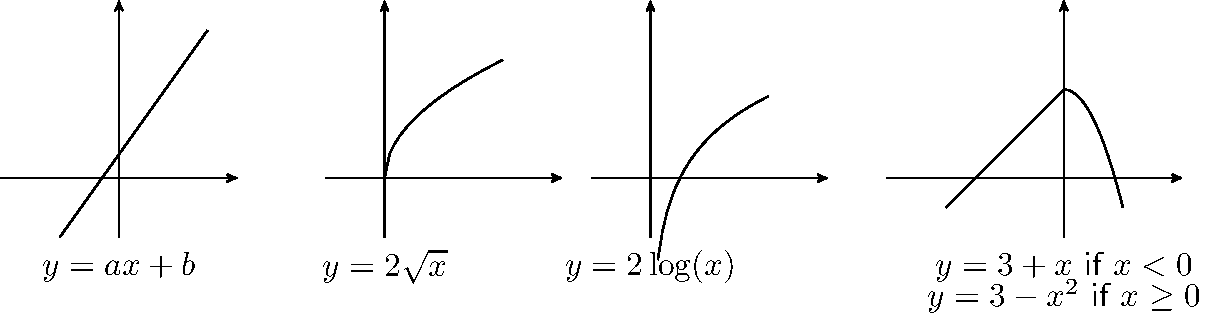
\includegraphics[width = \textwidth]{Chapters/08_ConvexOptimization/16_convexity/latex/concavefunctions.pdf}
    \caption[]{Ví dụ về các hàm lõm một biến.}
    \label{fig:16_concavefunctions}
    \captionsetup[figure]{format=rule, justification=centering}
    % \myrule
\end{figure}
% ******************************************************************************
 
\index{hàm affine -- affine function}
\subsubsection{Hàm affine}
\textit{Hàm affine} là tổng của một hàm tuyến tính và một hằng số, tức là các hàm có dạng $f(\mathbf{x}) = \mathbf{a}^T\mathbf{x} + b $. 
 
Khi biến là một ma trận $\mathbf{X}$, các hàm affine được định nghĩa: 
\begin{equation*} 
f(\mathbf{X}) = \text{trace}(\mathbf{A}^T\mathbf{X}) + b 
\end{equation*} 
trong đó, $\mathbf{A}$ là một ma trận có cùng kích thước như $\mathbf{X}$
để đảm bảo phép nhân ma trận thực hiện được và kết quả là một ma trận vuông.
Các hàm affine vừa lồi vừa lõm. 

\index{dạng toàn phương -- quadratic form} 
\subsubsection{Dạng toàn phương}
Đa thức bậc hai một biến có dạng $f(x) = a x^2 + bx + c$ là lồi nếu $a > 0$, là lõm nếu $a < 0$. 
 
Khi biến là một vector $\mathbf{x} = [x_1, x_2, \dots, x_n]$, \textit{dạng
toàn phương} ({quadratic form}) là một hàm số có dạng
\begin{equation*} 
f(\mathbf{x}) = \mathbf{x}^T\mathbf{A}\mathbf{x} + \mathbf{b}^T\mathbf{x} + c 
\end{equation*} 
với $\mathbf{A}$ là một ma trận đối xứng và $\bx$ là vector có chiều phù hợp. 

Nếu $\mathbf{A}$ là một ma trận nửa xác định dương thì $f(\mathbf{x})$ là một
hàm lồi. Nếu $\mathbf{A}$ là một ma trận nửa xác định âm, $f(\mathbf{x})$
là một hàm lõm.
 
Nhắc lại hàm mất mát trong hồi quy tuyến tính:
% \begin{equation*} 
\begin{eqnarray*} 
\mathcal{L}(\mathbf{w}) &=& \frac{1}{2N} \|\mathbf{y} -
\bX^T\mathbf{w}\|_2^2 = \frac{1}{2N} (\mathbf{y} -
\mathbf{X}^T\mathbf{w})^T(\mathbf{y} - \mathbf{X}^T\mathbf{w})  \\\ 
&=& \frac{1}{2N} \mathbf{w}^T\mathbf{X}\bX^T\bw -
\frac{1}{N}\mathbf{y}^T\mathbf{X}^T\bw + \frac{1}{2N}\mathbf{y}^T\mathbf{y}.
\end{eqnarray*} 
% \end{equation*} 
Vì $\mathbf{X}\mathbf{X}^T$ là một ma trận nửa xác định dương, hàm mất mát của
hồi quy tuyến tính là một hàm lồi.
 
 
\subsubsection{Chuẩn}
Mọi hàm số bất kỳ thỏa mãn ba điều kiện của chuẩn đều là hàm số lồi. Việc này có thể
được trực tiếp suy ra từ bất đẳng thức tam giác của một chuẩn. 


Hình~\ref{fig:16_norm_surf} minh hoạ hai ví dụ về bề mặt của chuẩn $\ell_1$ và
$\ell_2$
trong không gian hai chiều (chiều thứ ba là giá trị của hàm
số). Nhận thấy các bề mặt này đều có {một đáy duy nhất} tại gốc tọa độ (đây chính là điều kiện đầu tiên của chuẩn). 

% Điều này cho thấy nếu
% ta {thả một hòn bi} ở vị trí bất kỳ trên các bề mặt này, cuối cùng nó sễ
% \textit{lăn} về đáy. Nếu liên tưởng tới thuật toán gradient descent thì việc áp
% dụng thuật toán này vào các bài toán không ràng buộc với hàm mục tiêu là
% strictly convex (và giả sửa là khả vi, tức có đạo hàm) sẽ cho kết quả rất tốt
% với learning rate phù hợp. Tính chất này khiến cho các hàm convex và strictly
% convex được đặc biệt quan tâm trong tối ưu. 

% ******************************************************************************
\begin{figure}[t]
    \begin{subfigure}{0.48\textwidth}
    % 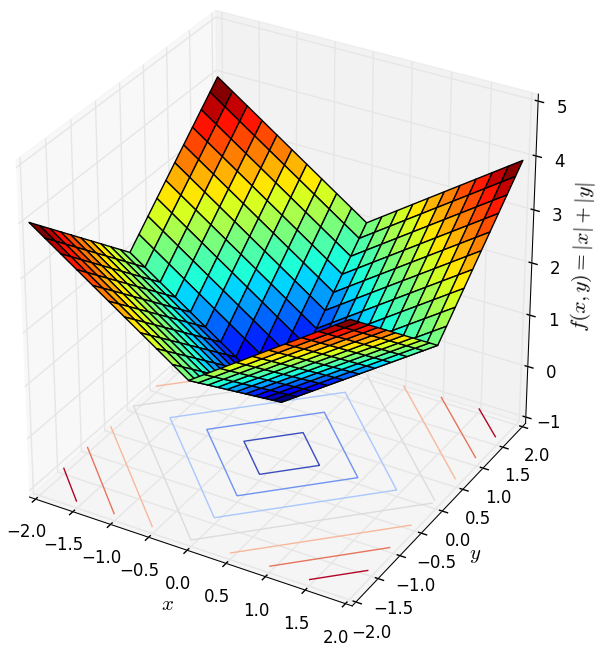
\includegraphics[width=0.999\linewidth]{Chapters/08_ConvexOptimization/16_convexity/norm1_surf.png}
    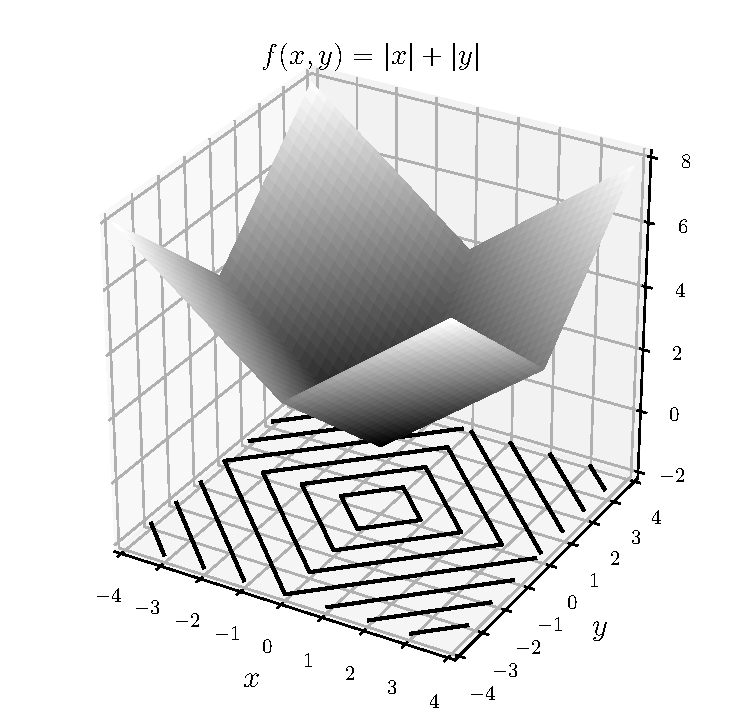
\includegraphics[width=0.999\linewidth]{ebookML_src/src/convexity/norm1_surf.pdf}
    \caption{Norm 1}
    \label{fig:subim1}
    \end{subfigure}
    \begin{subfigure}{0.48\textwidth}
    % 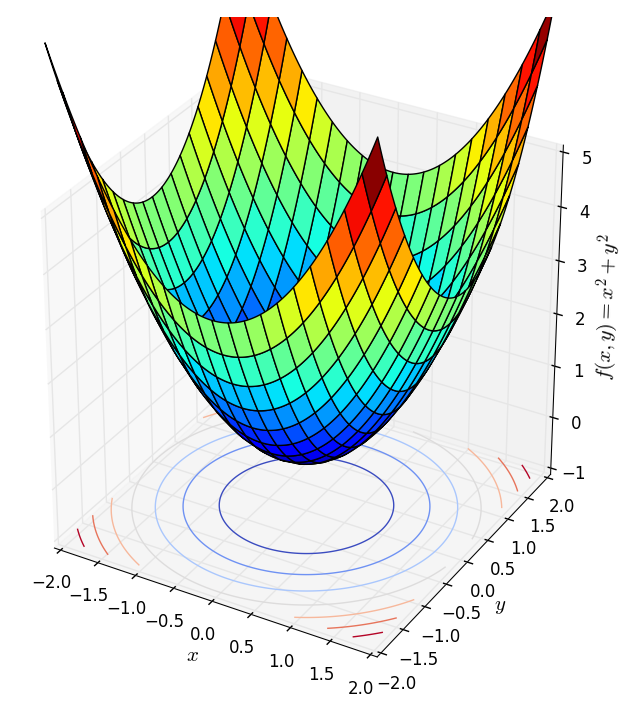
\includegraphics[width=0.999\linewidth]{Chapters/08_ConvexOptimization/16_convexity/norm2_surf.png}
    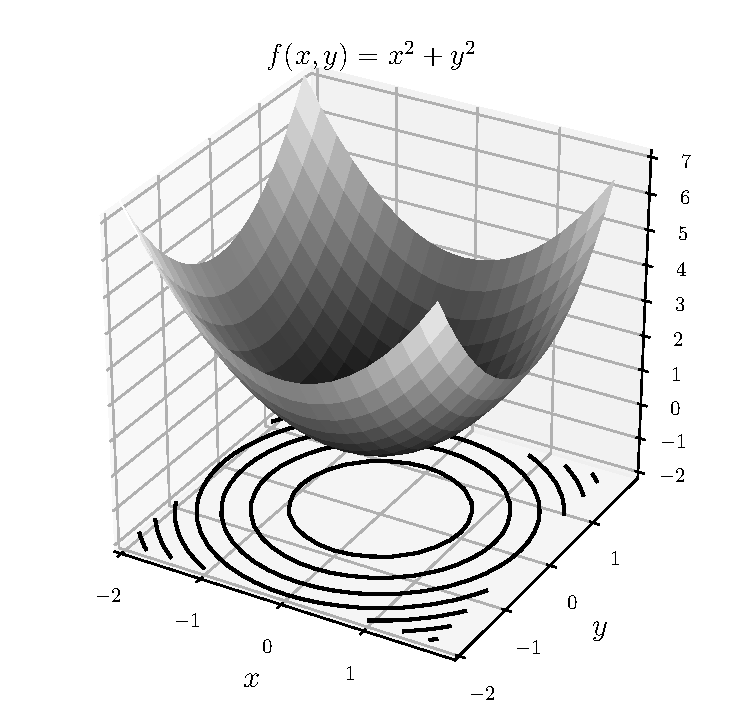
\includegraphics[width=0.999\linewidth]{ebookML_src/src/convexity/norm2_surf.pdf}
    \caption{Norm 2}
    \label{fig:subim2}
    \end{subfigure}
    \caption{Ví dụ về mặt của các chuẩn của vector hai chiều.}
    \label{fig:16_norm_surf}
\end{figure}
% ******************************************************************************
Hai hàm tiếp theo là ví dụ về các hàm không lồi hoặc lõm. Hàm
thứ nhất $f(x, y) = x^2 - y^2$ là một hyperbolic, hàm thứ hai $f(x,y) =
\frac{1}{10}(x^2 + 2y^2 - 2\sin(xy)) $. Các bề mặt của hai hàm này được minh
họa trên Hình~\ref{fig:16_nonconvexsurface}
 
 
 
% ******************************************************************************
\begin{figure}[t]
    \begin{subfigure}{0.48\textwidth}
    % 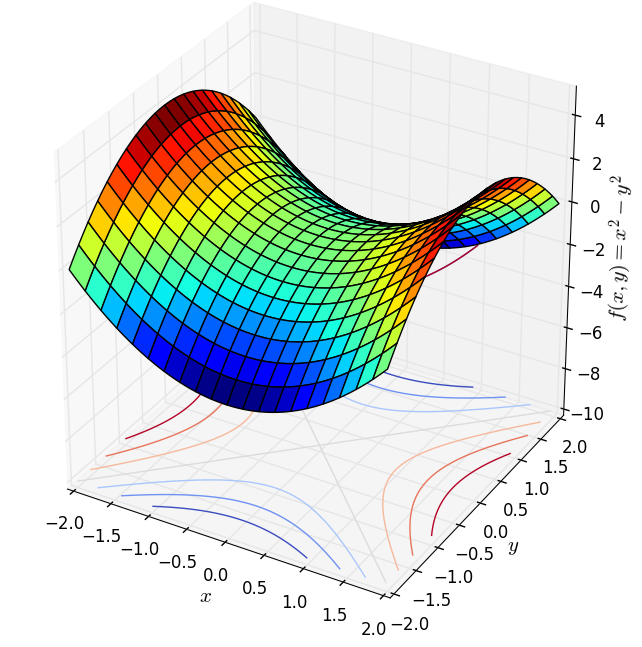
\includegraphics[width=0.95\linewidth]{Chapters/08_ConvexOptimization/16_convexity/hyperbol.png}
    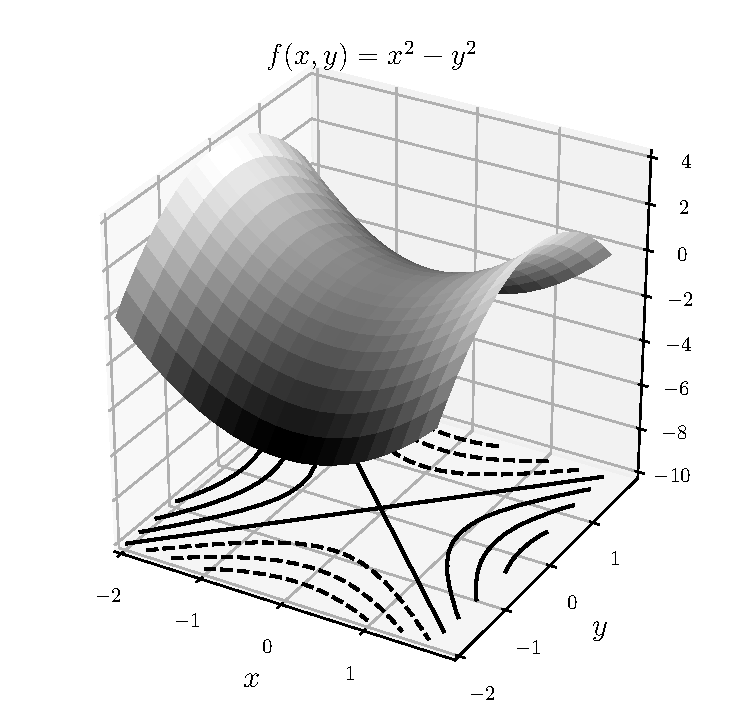
\includegraphics[width=0.95\linewidth]{ebookML_src/src/convexity/hyperbol.pdf}
    % \caption{Norm 1}
    % \label{fig:subim1}
    \end{subfigure}
    \begin{subfigure}{0.48\textwidth}
    % 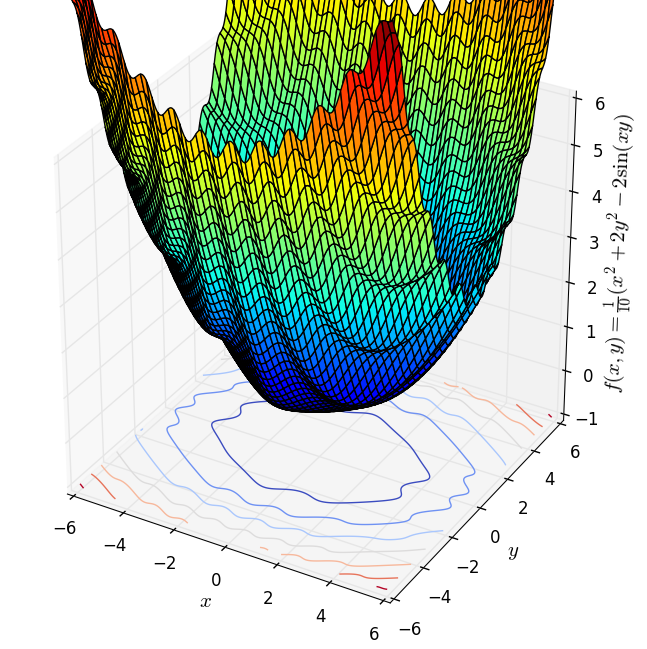
\includegraphics[width=0.95\linewidth]{Chapters/08_ConvexOptimization/16_convexity/nonconvex_surface.png}
    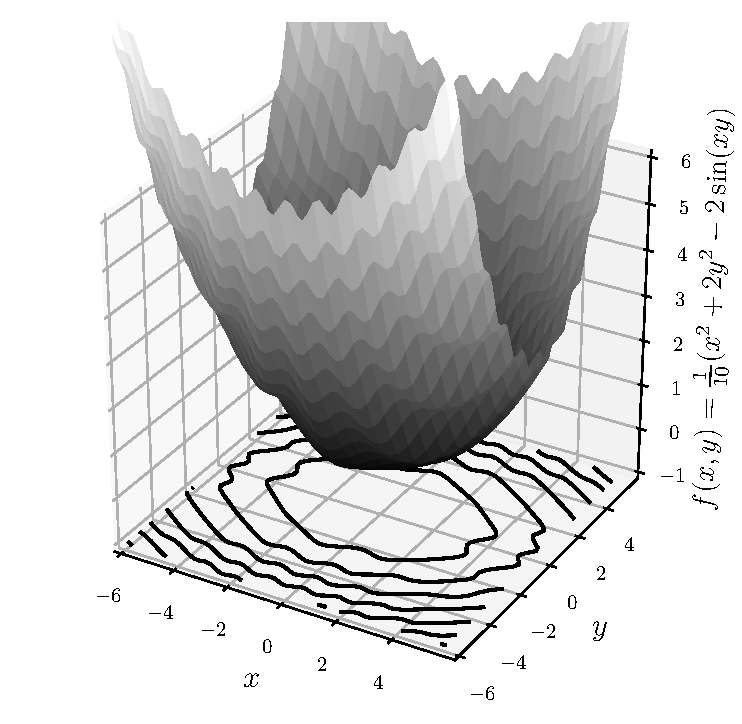
\includegraphics[width=0.95\linewidth]{ebookML_src/src/convexity/nonconvex_surface.pdf}
    % \caption{Norm 2}
    % \label{fig:subim2}
    \end{subfigure}
    \caption{Ví dụ về các hàm hai biến không lồi. }
    \label{fig:16_nonconvexsurface}
\end{figure}
% ******************************************************************************

\index{duo@đường đồng mức -- level sets}
\subsection{Đường đồng mức} 
Để khảo sát tính lồi của các bề mặt trong không gian ba chiều, việc minh hoạ
trực tiếp như các ví dụ trên đây có thể khó tưởng tượng hơn. Một phương pháp
thường được sử dụng là dùng các \textit{đường đồng mức} ({contour} hay
{level set}). Đường đồng mức là cách mô tả các mặt ở không gian ba chiều
trong không gian hai chiều. Ở đó, các điểm thuộc cùng một {đường} tương
ứng với các điểm làm cho hàm số có giá trị như nhau. Trong Hình~\ref{fig:16_norm_surf} và Hình
\ref{fig:16_nonconvexsurface}, các đường nối liền ở mặt phẳng đáy $0xy$
chính là các đường đồng mức. Nói cách khác, nếu cắt bề mặt bởi các mặt phẳng song song với đáy, ta sẽ thu được các đường đồng mức.

%******************************************************************************
\begin{figure}[t]
    \begin{subfigure}{0.325\textwidth}
        % 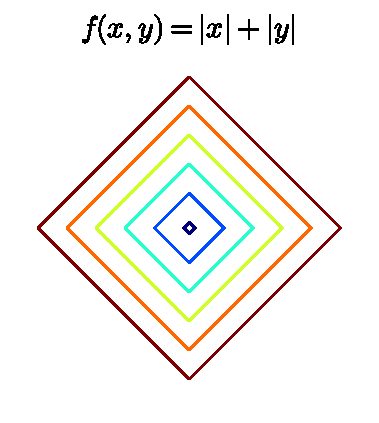
\includegraphics[width=0.99\linewidth]{Chapters/08_ConvexOptimization/16_convexity/python/abs_2d.pdf}
        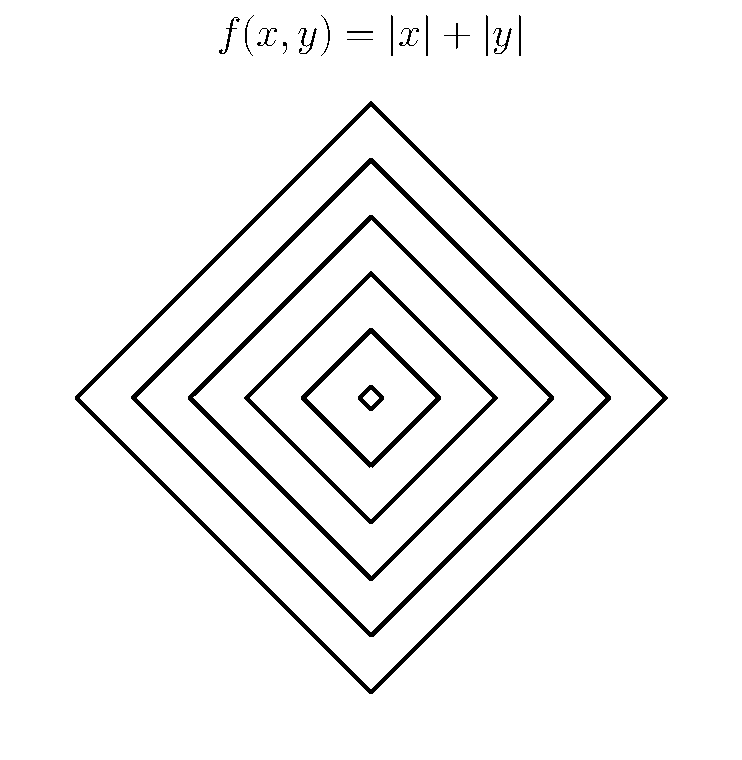
\includegraphics[width=0.99\linewidth]{ebookML_src/src/convexity/abs_2d.pdf}
        \caption{}
    \end{subfigure}
    \begin{subfigure}{0.325\textwidth}
        % 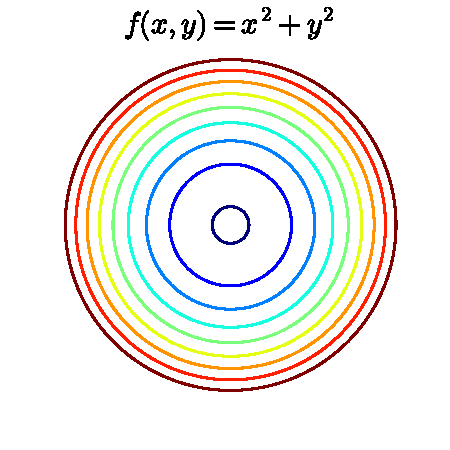
\includegraphics[height=1.02\linewidth]{Chapters/08_ConvexOptimization/16_convexity/python/norm_2d.pdf}
        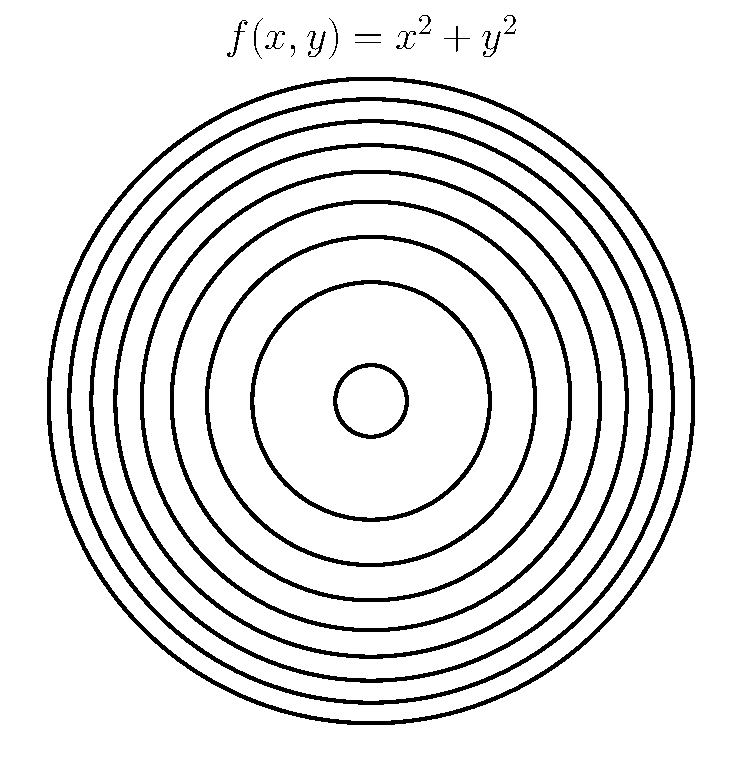
\includegraphics[height=1.02\linewidth]{ebookML_src/src/convexity/norm_2d.pdf}
        \caption{}
    \end{subfigure}
    \begin{subfigure}{0.325\textwidth}
        % 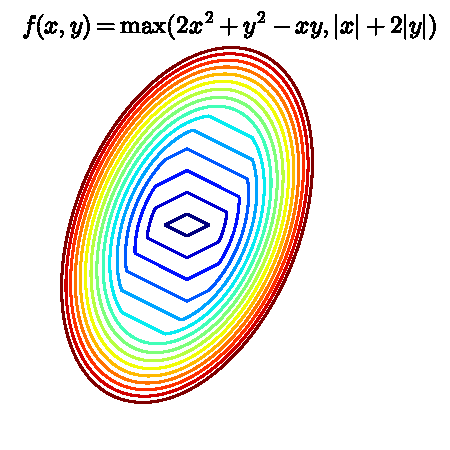
\includegraphics[height=1.02\linewidth]{Chapters/08_ConvexOptimization/16_convexity/python/max_2d.pdf}
        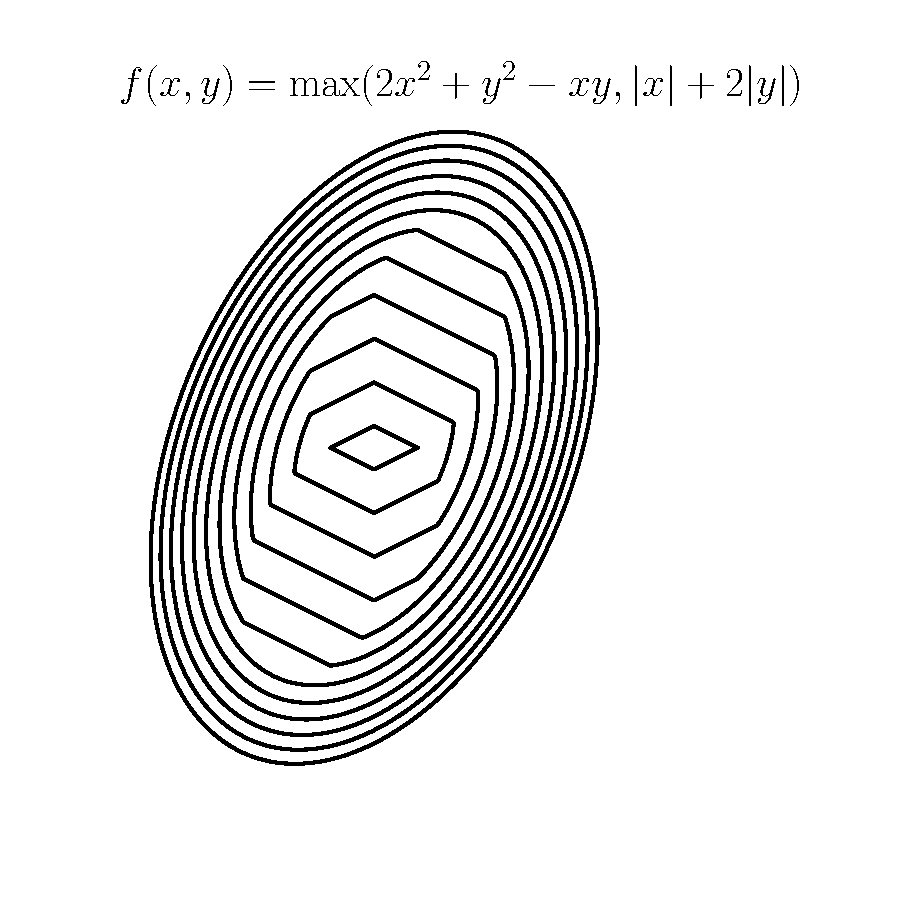
\includegraphics[height=1.02\linewidth]{ebookML_src/src/convexity/max_2d.pdf}
        \caption{}
    \end{subfigure}

    \begin{subfigure}{0.325\textwidth}
        % 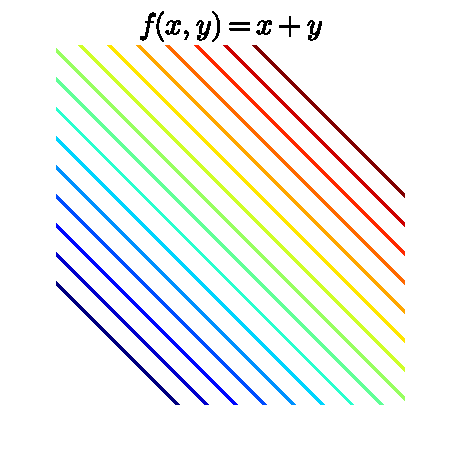
\includegraphics[height=1.02\linewidth]{Chapters/08_ConvexOptimization/16_convexity/python/linear_2d.pdf}
        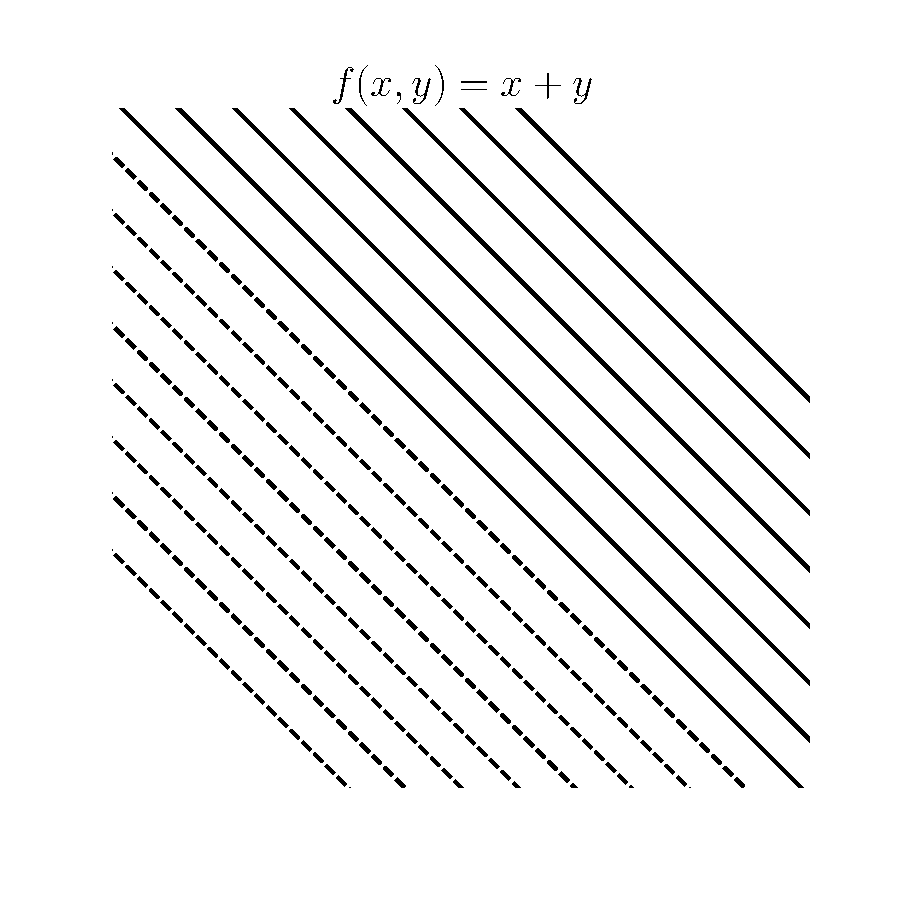
\includegraphics[height=1.02\linewidth]{ebookML_src/src/convexity/linear_2d.pdf}
        \caption{}
        \label{fig:16_contoursd}
    \end{subfigure}
    \begin{subfigure}{0.325\textwidth}
        % 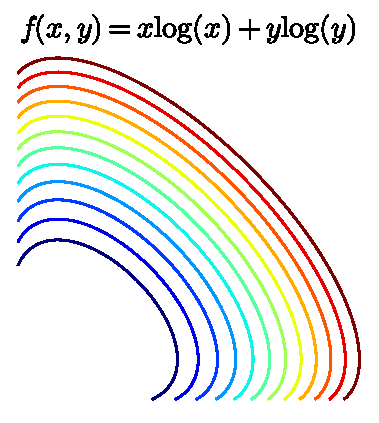
\includegraphics[height=1.02\linewidth]{Chapters/08_ConvexOptimization/16_convexity/python/NE.pdf}
        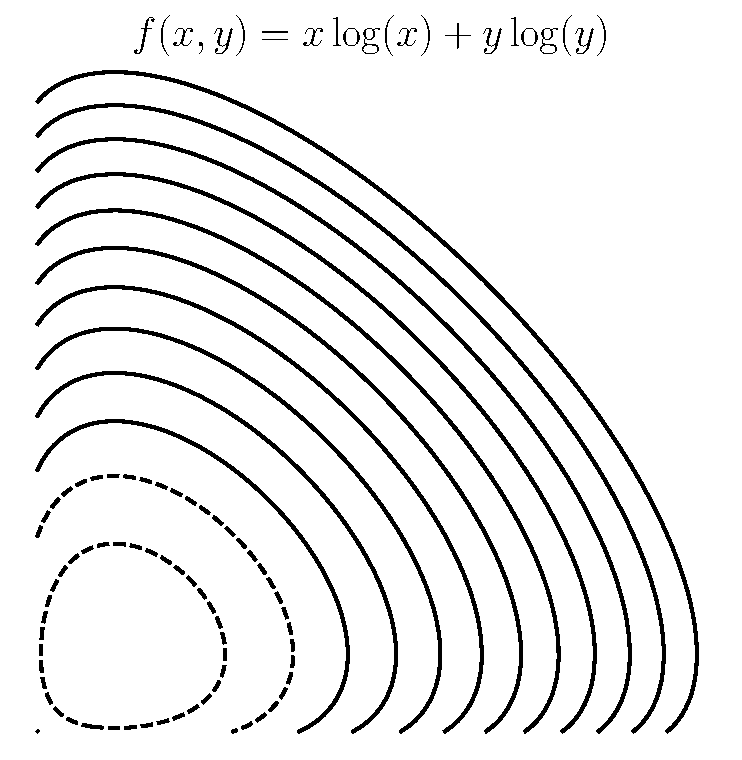
\includegraphics[height=1.02\linewidth]{ebookML_src/src/convexity/NE.pdf}
        \caption{}
        \label{fig:16_contourse}
    \end{subfigure}
    \begin{subfigure}{0.325\textwidth}
        % 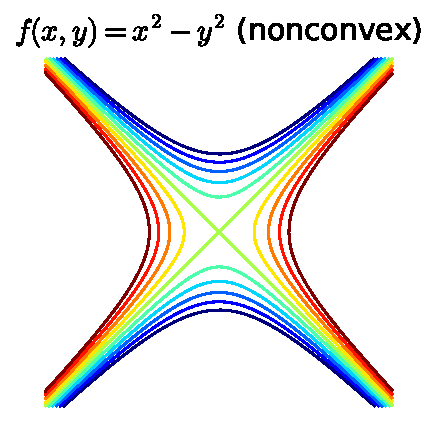
\includegraphics[height=1.02\linewidth]{Chapters/08_ConvexOptimization/16_convexity/python/hyper_2d.pdf}
        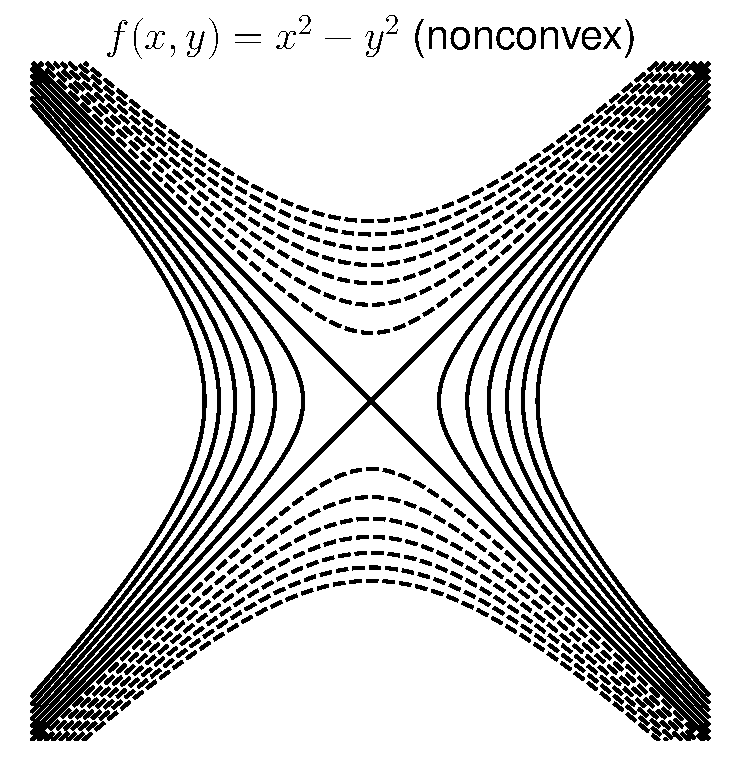
\includegraphics[height=1.02\linewidth]{ebookML_src/src/convexity/hyper_2d_2.pdf}
        \caption{}
        \label{fig:16_contoursf}
    \end{subfigure}
    \caption{Ví dụ về đường đồng mức. Hàng trên: các đường đồng mức càng gần tâm tương ứng với các giá trị càng nhỏ. Hàng dưới: các đường nét đứt tương ứng với các giá trị âm, các đường nét liền tương ứng với các giá trị không âm. Các hàm số đều lồi ngoại trừ hàm số trong hình f).}
    \label{fig:16_contours}
\end{figure}
% ******************************************************************************
 
Khi khảo sát tính lồi hoặc tìm điểm cực trị của một hàm hai biến,
người ta thường vẽ các đường đồng mức thay vì các bề mặt trong không gian ba chiều.
Hình~\ref{fig:16_contours} minh hoạ một vài ví dụ về đường đồng mức. Ở hàng trên,
các đường đồng mức là các đường khép kín. Khi các đường này co dần lại ở một điểm thì điểm đó là điểm cực trị. Với các hàm
lồi như trong ba ví dụ này, chỉ có một điểm cực trị và đó cũng là điểm cực trị toàn cục. Nếu để ý, bạn sẽ thấy các
đường khép kín tạo thành biên của các {tập lồi}. Ở hàng dưới, các đường
không khép kín. Hình~\ref{fig:16_contoursd} minh hoạ các đường đồng mức của một
hàm tuyến tính $f(x, y) = x + y$, và là một hàm lồi.
Hình~\ref{fig:16_contourse} minh hoạ các đường đồng mức của một hàm lồi (chúng
ta sẽ sớm chứng minh) nhưng các đường đồng mức không kín.
Hàm này có chứa $\log$ nên tập xác định là góc phần tư thứ nhất tương ứng với tọa độ dương (chú ý rằng tập hợp điểm có tọa độ dương cũng là một
{tập lồi} vì nó là một siêu đa diện). Các {đường không kín} này nếu
kết hợp với trục $Ox, Oy$ sẽ tạo thành biên của các {tập lồi}.
Hình~\ref{fig:16_contoursf} minh hoạ các đường đồng mức của một hàm hyperbolic, hàm
này không phải là một hàm lồi.
 
\index{tập dưới mức $\alpha$ -- $\alpha$-sublevel set} 
\subsection{Tập dưới mức $\alpha$}
% \myrule 

\begin{mydef}{Tập dưới mức $\alpha$}{alphasub}
    
 Tập dưới mức $\alpha$ ($\alpha$-sublevel set) của một hàm số $f : \mathbb{R}^n \rightarrow
 \mathbb{R}$ là một tập hợp được định nghĩa bởi
\begin{equation*} 
\mathcal{C}_{\alpha} = \{\mathbf{x} \in \text{\bf dom} f ~\big|~ f(\mathbf{x}) \leq \alpha\} 
\end{equation*} 
\end{mydef}
% \myrule 
Diễn đạt bằng lời, một tập dưới mức $\alpha$ của một hàm số $f(.)$ là tập hợp các
điểm trong tập xác định của $f(.)$ mà tại đó hàm số đạt giá trị không lớn hơn
$\alpha$.
 
 
Quay lại với Hình \ref{fig:16_contours}, hàng trên, tập dưới mức $\alpha$ là các hình lồi được bao bởi đường đồng mức. Trong Hình~\ref{fig:16_contoursd}, tập dưới mức $\alpha$ là phần nửa mặt phẳng phía dưới xác định bởi
các đường thẳng đồng mức. Trong Hình~\ref{fig:16_contourse}, tập dưới mức $\alpha$ là vùng bị giới hạn bởi các trục tọa độ và các đường đường đồng mức. Trong
Hình~\ref{fig:16_contoursf}, tập dưới mức $\alpha$ hơi khó tưởng tượng hơn. Với $\alpha > 0$, đường đồng mức là các đường nét liền, các tập dưới mức
$\alpha$ tương ứng là phần nằm giữa các đường nét liền này. Có thể
nhận thấy các vùng này không phải là tập lồi.

\begin{mytheo}{}{alphasub}
Nếu một hàm số là lồi thì {mọi} tập dưới mức $\alpha$
của nó lồi. Điều ngược lại chưa chắc đã đúng, tức nếu các tập dưới mức $\alpha$ của một hàm số là \textit{lồi} thì hàm số đó chưa chắc đã \textit{lồi}. 
\end{mytheo}    

 
Điều này chỉ ra rằng nếu tồn tại một giá trị $\alpha$ sao cho một tập dưới mức 
$\alpha$ của một hàm số là \textit{không lồi}, thì hàm số đó {không lồi}. Vì vậy, hàm hyperbolic không phải là một hàm
lồi. Các ví dụ trong Hình~\ref{fig:16_contours}, trừ Hình~\ref{fig:16_contoursf},
đều tương ứng với các hàm lồi.
 
Xét ví dụ về việc một hàm số không lồi nhưng mọi
tập dưới mức $\alpha$ đều lồi. Hàm $f(x, y) = -e^{x+y}$ có mọi tập dưới mức 
$\alpha$ là một nửa mặt phẳng (lồi), nhưng nó
không phải là một hàm lồi (trong trường hợp này nó là một hàm lõm).
 
% ******************************************************************************
\begin{figure}[t]
\centering
    % 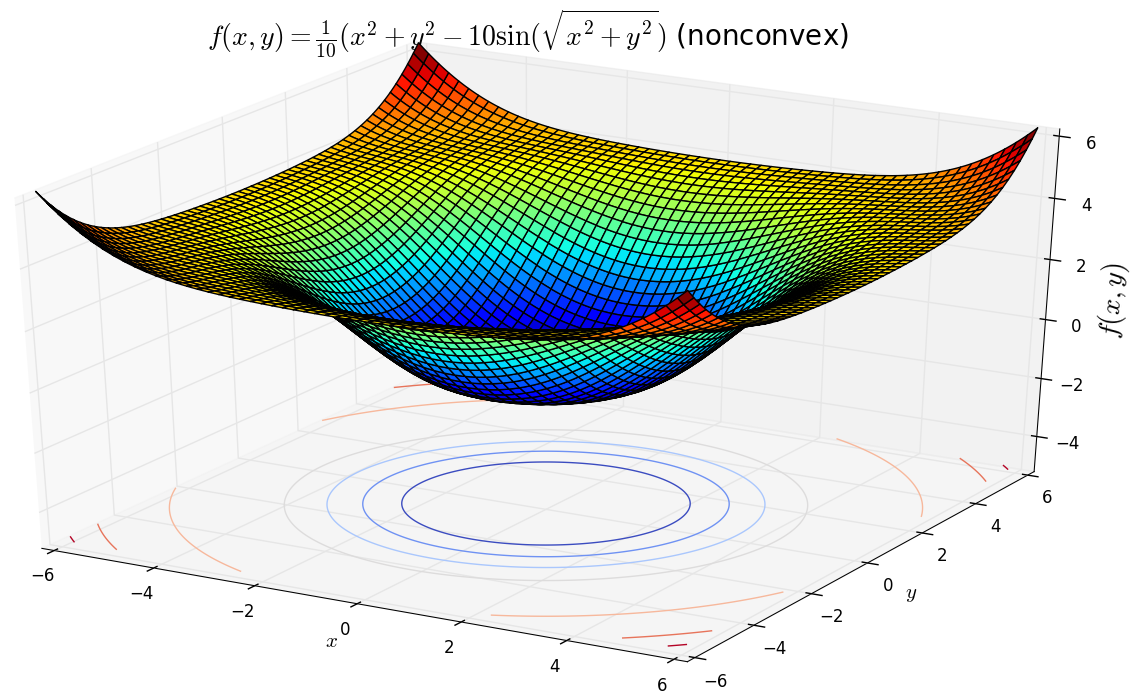
\includegraphics[width = .8\textwidth]{Chapters/08_ConvexOptimization/16_convexity/sin_surf2_cropped.png}
    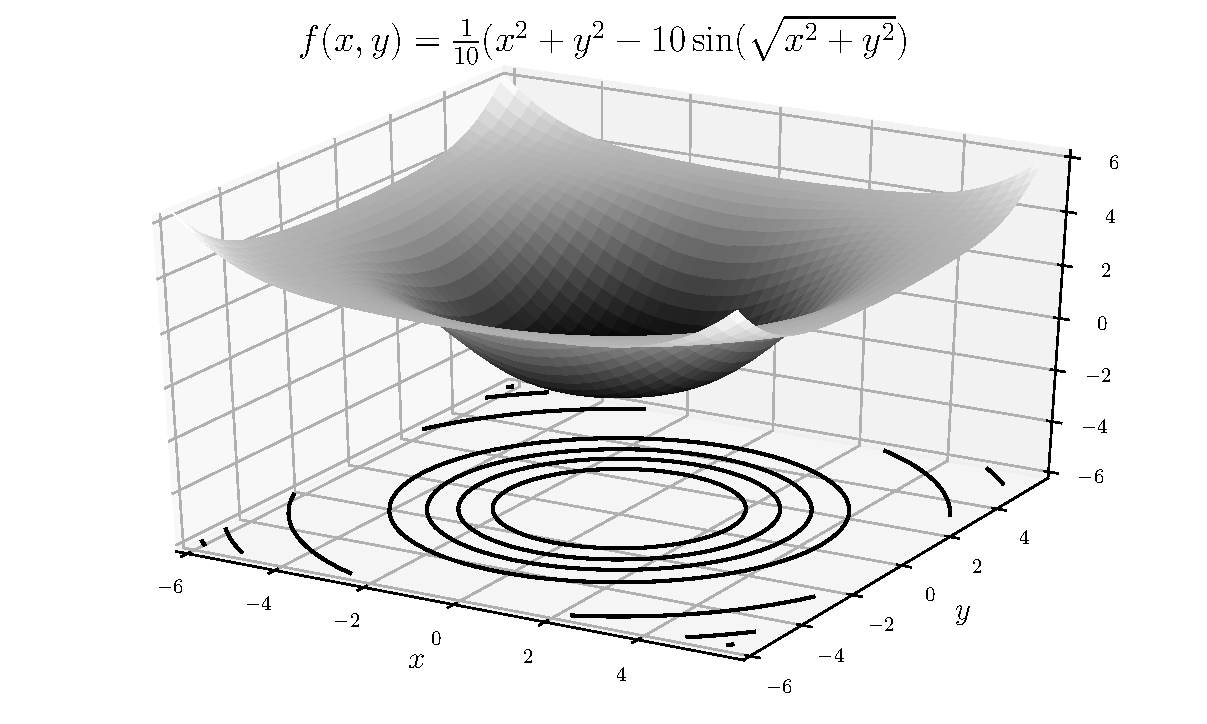
\includegraphics[width = .8\textwidth]{ebookML_src/src/convexity/sin_surf2_cropped.pdf}
    \caption[]{Mọi tập dưới mức $\alpha$ là tập lồi nhưng hàm số là không lồi.}
    \label{fig:16_ex}
\end{figure}
% ******************************************************************************

Hình~\ref{fig:16_ex} là một ví dụ khác về việc một hàm số có mọi tập dưới mức
$\alpha$ {lồi} nhưng không phải là một hàm lồi. Mọi tập dưới mức
$\alpha-$ của hàm số này đều là hình tròn  --  lồi, nhưng
hàm số đó không {lồi}. Vì có thể tìm được hai điểm trên mặt này
sao cho đoạn thẳng nối chúng nằm hoàn toàn phía dưới của mặt. Chẳng hạn,
đoạn thẳng nối một điểm ở
{cánh} và một điểm ở {đáy} không nằm hoàn toàn phía trên của mặt.
% \tcb{stop here}
Những hàm số có tập xác định là một {tập lồi} và có mọi tập dưới mức $\alpha$
là lồi được gọi là  \textit{hàm tựa lồi} (quasiconvex function). Mọi hàm lồi đều là tựa lồi nhưng ngược lại không đúng. Định nghĩa chính thức của
hàm tựa lồi được phát biểu như sau
\index{tựa lồi -- quasiconvex}

\begin{mydef}{Hàm tựa lồi}{quasiconvex}
Một hàm số $f: \mathcal{C} \rightarrow \mathbb{R}$ với $\mathcal{C}$ là một tập con {lồi} của $\mathbb{R}^n$ được gọi là \textit{tựa lồi} (quasiconvex) nếu với mọi $\mathbf{x}, \mathbf{y} \in \mathcal{C}$ và mọi $\theta \in [0, 1]$, ta có:  
\begin{equation*} 
f(\theta\mathbf{x} + (1 - \theta)\mathbf{y}) \leq \max\{f(\mathbf{x}), f(\mathbf{y})\} 
\end{equation*} 
\end{mydef}

% Định nghĩa này khác với định nghĩa về \textit{convex function} một chút ở việc
% sử dụng hàm max.
 
% \tcr{stop }
 
\subsection{Kiểm tra tính chất lồi dựa vào đạo hàm}
Ta có thể nhận biết một hàm số khả vi có là hàm lồi hay không dựa vào các
đạo hàm bậc nhất hoặc bậc hai của nó. Giả sử rằng các
đạo hàm đó tồn tại. 

\index{die@điều kiện bậc nhất -- first-order condition}
\subsubsection{Điều kiện bậc nhất}

Trước hết chúng ta định nghĩa phương trình (mặt) tiếp tuyến của một hàm số
$f$ khả vi tại một điểm nằm trên đồ thị (mặt) của hàm số đó $(\mathbf{x}_0,
f(\mathbf{x}_0)$. Với hàm một biến, phương trình tiếp tuyến tại điểm có tọa độ
$(x_0, f(x_0))$ là 
\begin{equation*} 
y = f'(x_0)(x - x_0) + f(x_0) 
\end{equation*} 
Với hàm nhiều biến, đặt $\nabla f(\mathbf{x}_0)$ là gradient của hàm số $f$ tại điểm $\mathbf{x}_0$, phương trình mặt tiếp tuyến được cho bởi: 
\begin{equation*} 
y = \nabla f(\mathbf{x}_0)^T (\mathbf{x} - \mathbf{x}_0) + f(\mathbf{x}_0) 
\end{equation*} 

    

\newnote{Điều kiện bậc nhất}{Giả sử hàm số $f$ {có tập xác định là
lồi} và có đạo hàm tại mọi điểm trên tập xác định đó. Khi đó, hàm số $f$ 
\textit{lồi} {khi và chỉ khi} với mọi $\mathbf{x}, \mathbf{x}_0$ trên tập
xác định, ta có:
\begin{equation} 
\label{eqn:16_firstorder}
f(\mathbf{x}) \geq f(\mathbf{x}_0) + \nabla f(\mathbf{x}_0)^T(\mathbf{x} - \mathbf{x}_0)
\end{equation} 
}
 
Một hàm số là lồi chặt nếu dấu bằng trong \eqref{eqn:16_firstorder} xảy ra khi và chỉ khi $\mathbf{x} = \mathbf{x}_0$. 
 
Một cách trực quan hơn, một hàm số là lồi nếu mặt tiếp tuyến tại một điểm
bất kỳ \textit{không nằm phía trên} mặt đồ thị của hàm số đó.



% \myrule  
% <div class="imgcap"> 
%  <img src ="/assets/16_convexity/first_order.png" align = "center" width = "800"> 
%  <div class = "thecap">Hình 13. Kiểm tra tính convexity dựa vào đạo hàm bậc nhất. Trái: hàm lồi, phải: hàm không lồi.</div> 
% </div> 
% \myrule  

\begin{figure}[t]
\centering
    % 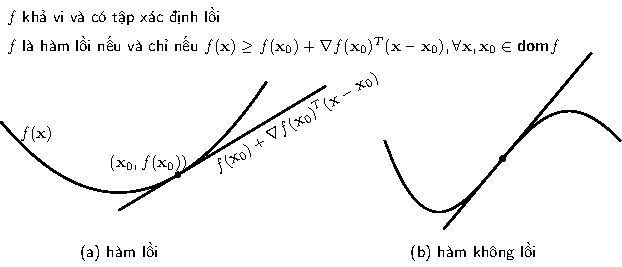
\includegraphics[width = \textwidth]{Chapters/08_ConvexOptimization/16_convexity/latex/first_order.pdf}
    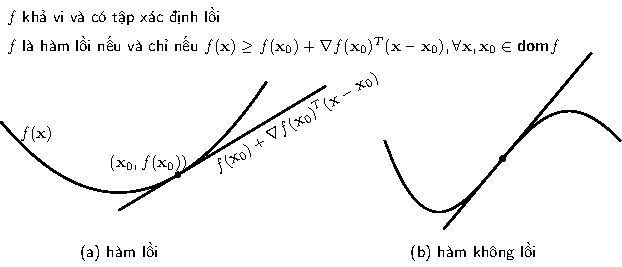
\includegraphics[width = \textwidth]{Chapters/08_ConvexOptimization/16_convexity/latex/first_order.pdf}
    \caption[]{Kiểm tra tính lồi dựa vào đạo hàm bậc nhất. Trái: hàm lồi vì tiếp tuyến tại mọi điểm đều nằm phía dưới đồ thị của hàm số, phải: hàm không lồi.}
    \label{fig:16_firstorder}
\end{figure}

Hình~\ref{fig:16_firstorder} minh hoạ đồ thị của một hàm lồi và một hàm không
lồi. Hình~\ref{fig:16_firstorder}a mô tả một hàm lồi.
Hình~\ref{fig:16_firstorder}b mô tả một hàm không lồi vì đồ thị của nó không hoàn toàn nằm phía trên đường thẳng tiếp tuyến.
 
\textit{Ví dụ}: $f(\mathbf{x}) = \mathbf{x}^T\mathbf{A}\mathbf{x}$ là một hàm lồi nếu  $\mathbf{A}$ là một ma trận {nửa xác định dương}. 
 
\textit{Chứng minh:} Đạo hàm bậc nhất của $f(\bx)$ là 
\begin{math} 
\nabla f(\mathbf{x}) = 2\mathbf{A} \mathbf{x} 
\end{math}.
Vậy điều kiện bậc nhất có thể viết dưới dạng (chú ý rằng $\mathbf{A}$ là một ma trận đối xứng): 
% \begin{equation*} 
\begin{eqnarray*} 
\mathbf{x}^T\mathbf{Ax} &\geq& 2(\mathbf{A}\mathbf{x}_0)^T (\mathbf{x} - \mathbf{x}_0) + \mathbf{x}_0^T\mathbf{A}\mathbf{x}_0 \\\ 
\Leftrightarrow \mathbf{x}^T\mathbf{Ax} &\geq& 2\mathbf{x}_0^T\mathbf{A}\mathbf{x} -\mathbf{x}_0^T\mathbf{A}\mathbf{x}_0  \\\ 
\Leftrightarrow (\mathbf{x} - \mathbf{x}_0)^T\mathbf{A}(\mathbf{x} - \mathbf{x}_0) &\geq& 0 
\end{eqnarray*} 
% \end{equation*} 
Bất đẳng thức cuối cùng đúng dựa trên định nghĩa của ma trận {nửa xác
định dương}. Vậy hàm số $f(\mathbf{x}) = \mathbf{x}^T\mathbf{A}\mathbf{x}$ là
một {hàm lồi}. \dpcm
 

\index{die@điều kiện bậc hai -- second-order condition}
\subsection{Điều kiện bậc hai}
\index{Hesse -- Hessian}
Với hàm có đối số là một vector có chiều $d$, đạo hàm bậc
nhất của nó là một vector cũng có chiều $d$. Đạo hàm bậc hai của nó là một ma
trận vuông có chiều $d\times d$.

\newnote{Điều kiện bậc hai} {Một hàm số $f$ có đạo hàm bậc hai là hàm lỗi nếu tập xác định của nó lồi và Hesse là một ma trận {nửa xác định dương} với mọi $\mathbf{x}$ trong tập xác định: 
\begin{equation*} 
\nabla^2 f(\mathbf{x}) \succeq 0. 
\end{equation*} 
}


Nếu Hesse của một hàm số là một ma trận {xác định dương} thì hàm số đó
lồi chặt. Tương tự, nếu Hesse là một ma trận {xác
định âm} thì hàm số đó lõm chặt.
 
Với hàm số một biến $f(x)$, điều kiện này tương đương với $f"(x) \geq 0$ với mọi
$x$ thuộc tập xác định (và tập xác định là lồi).
 
% \newpage 
\index{entropy chéo -- cross entropy}
\textit{Ví dụ:} 
\begin{itemize}
    \item Hàm $f(x) = x\log(x)$ là lồi chặt vì tập xác định $x > 0$ là một tập lồi và $f"(x) = 1/x$ là một số
    dương với mọi $x$ thuộc tập xác định.
    \item Xét hàm số hai biến: $f(x, y) = x
    \log(x) + y \log(y) $ trên tập các giá trị dương của $x$ và $y$. Hàm số này
    có đạo hàm bậc nhất $[\log(x) + 1, \log(y) + 1]^T$ và Hesse $\bmt
    1/x & 0 \\ 0 & 1/y
    \emt $ là một ma trận đường chéo xác định dương. Vậy đây là một hàm lồi chặt.
    
    \item Hàm $f(x) = x^2 + 5\sin(x)$ không là hàm lồi vì đạo hàm bậc hai $f"(x)
    = 2 - 5\sin(x)$ có thể nhận cả giá trị âm và dương.
     
    \item Hàm {entropy} chéo là một hàm lồi chặt. Xét hai xác suất $x$ và $1 - x$ ($0 < x < 1$), và $a$ là một hằng số thuộc
    đoạn $[0, 1]$: $f(x) = -(a \log(x) + (1 - a) \log(1 - x))$ có
    đạo hàm bậc hai $\frac{a}{x^2} + \frac{1 - a}{(1-x)^2}$ là một số dương.
     
    \item Nếu $\mathbf{A}$ là một ma trận xác định dương thì $f(\mathbf{x}) =
    \frac{1}{2}\mathbf{x}^T\mathbf{Ax}$ là lồi vì $\bA$ chính là Hesse của nó.
     
    

\end{itemize}
 
 
 
Ngoài ra còn nhiều tính chất thú vị của các {hàm lồi}, mời bạn đọc thêm Chương 3 của cuốn \textit{Convex Optimization}~\cite{boyd2004convex}.
 
 
\section{Tóm tắt}
\begin{itemize}
    \item Machine learning và tối ưu có quan hệ mật thiết với nhau. Trong
    tối ưu, tối ưu lồi là quan trọng nhất. 
     
    \item Mọi đoạn thẳng nối hai điểm bất kỳ của một tập lồi nằm trọn vẹn trong tập đó. Giao điểm của các tập lồi tạo thành một
    tập lồi. 

    \item Một hàm số là lồi nếu đoạn thẳng nối hai điểm bất kỳ trên đồ thì hàm
    số đó {không nằm phía dưới} đồ thị đó.
     
    \item Một hàm số khả vi là lồi nếu tập xác định của nó là lồi 
    và mặt tiếp tuyến tại một điểm bất kỳ {không nằm phía trên} đồ thị
    của hàm số đó.
     
    \item Các chuẩn là các hàm lồi, được sử dụng nhiều trong tối ưu. 
 
\end{itemize}
 
% \section{Tài liệu tham khảo}
 
% [1] \href{http://stanford.edu/~boyd/cvxbook/}{Convex Optimization} – Boyd and Vandenberghe, Cambridge University Press, 2004. 
 
 
